\documentclass[12pt, openany, oneside, a4paper, english, brazil]{abntex2}   % Padrão Abntex2

%***************************** PACOTES *********************************** %
%\usepackage[within=none]{newfloat}
\usepackage[utf8]{inputenc}		     % Codificacao do documento (conversão automática dos acentos)


%	Fonte
\usepackage[T1]{fontenc}		   	 % Selecao de codigos de fonte.
\usepackage[brazil]{babel}
\usepackage{lmodern}			     % Usa a fonte Latin Modern

%	Matemático e Gráfico
\usepackage{float}
\usepackage{graphics,graphicx}	     % pacotes para inserir figuras .eps ou .jpg
\graphicspath{{figuras/}{resultados/}}            % pasta de figuras
\usepackage{amssymb}           		 % pacote para fontes e simbolos matemáticos
\usepackage{longtable}          	 % possibilita inserir grandes tabelas
\usepackage{makecell}                % possibilita pular linhas nas tabelas
\usepackage{xcolor,colortbl,multirow} % permite textos e tabelas com cores
\usepackage{amsmath}           		 % pacote para equações
\usepackage{epstopdf}
\usepackage{ragged2e}
\usepackage{listings}
%\lstset{numbers=left, numberstyle=\tiny, stepnumber=1, numbersep=5pt, basicstyle=\scriptsize ,frame=tbrl}
\usepackage{etoolbox}
\usepackage{multicol}
%\usepackage{caption}
\usepackage[position=b,singlelinecheck=on]{subfig}

\floatstyle{plaintop}
\newfloat{quadro}{htbp}{loq}
\floatname{quadro}{Quadro}

\makeatletter
\patchcmd{\listof}% <cmd>
{\float@listhead}% <search>
{\@namedef{l@#1}{\l@table}\float@listhead}% <replace>
{}{}% <success><failure>
\makeatother

%\makeatletter
%\renewcommand*{\float@listhead}[1]{%
%	\@ifundefined{chapter}{%
%		\section*{#1}%
%		\addcontentsline{toc}{section}{#1}%
%	}{%
%	\chapter*{#1}% 
%	\addcontentsline{toc}{chapter}{#1}%
%}%
%\@mkboth{\MakeUppercase{#1}}{\MakeUppercase{#1}}%
%}
%\makeatother




%\DeclareFloatingEnvironment{quadro}[Quadro][Lista de quadros]
%\DeclareCaptionType{quadro}[Quadros][Lista de quadros]


% % % % % % % % % % % % % % % % % % % %

\definecolor{codegreen}{rgb}{0,0.6,0}
\definecolor{codegray}{rgb}{0.5,0.5,0.5}
\definecolor{codepurple}{rgb}{0.58,0,0.82}
\definecolor{backcolour}{rgb}{0.95,0.95,0.92}

%\definecolor{verde}{rgb}{0,0,0}

\lstdefinestyle{mystyle}{
	backgroundcolor=\color{backcolour},   
	commentstyle=\color{codegreen},
	keywordstyle=\color{magenta},
	numberstyle=\tiny\color{codegray},
	stringstyle=\color{codepurple},
	basicstyle=\footnotesize,
	breakatwhitespace=false,         
	breaklines=true,                 
	captionpos=b,                    
	keepspaces=true,                 
	numbers=left,                    
	numbersep=5pt,                  
	showspaces=false,                
	showstringspaces=false,
	showtabs=false,                  
	tabsize=2
}

\lstset{style=mystyle}

%	Estrutural
\usepackage{url}
\usepackage{threeparttable}     	 % permite a inserção de notas de rodapé nas tabelas
\usepackage{lscape}             	 % orientação de página LANDSCAPE
\usepackage{pifont}             	 % acrescenta símbolos diferentes.
%\usepackage{cmap}					 % Mapear caracteres especiais no PDF	
\usepackage{lastpage}				 % Usado pela Ficha catalográfica
\usepackage{indentfirst}			 % Indenta o primeiro parágrafo de cada sessão.



% Pacotes de citações
%\usepackage[brazilian,hyperpageref]{backref}	 % Paginas com as citações na bibl
\usepackage[num,abnt-etal-text=it]{abntex2cite}	% Citações padrão ABNT numerica
\citebrackets[]
% remover bordas dos links
\hypersetup{
    colorlinks,
    linkcolor={black},
    citecolor={black},
    urlcolor={black}
} % resto dos pacotes Latex
%\usepackage[english]{style/UFSC-ECA-Monograph} % personalização da ABNTEX2 para escrita em inglês  
\usepackage[english]{style/UFSC-ECA-Monograph} % personalização da ABNTEX2 para escrita em português


%---------------------------------------------------------------
%--------- DADOS BÁSICOS DO TRABALHO (Preencher todos) ---------
%---------------------------------------------------------------


\titulo{Comparação e \textit{benchmarking} para SLAM em robôs móveis}   % Título do Trabalho em Português
\tituloingles{Comparison and benchmarking for SLAM in mobile robots}   % Título do Trabalho em Inglês

\DEELautor{Brunno}{Vanelli} % Aluno autor do trabalho

\curso{Engenharia de Controle e Automação}											
\orientador{Prof. Dr. Marcelo Roberto Petry}  % Professor Orientador membro da banca 

\membrob{Prof. Dr. Leonardo Mejia Rincon}   % Professor membro da banca 
\membroc{Prof. Dr. Ciro André Pitz}   % Professor membro da banca

\local{Blumenau}   % Cidade da instituição
\data{2019}        % Ano de realização


%--------------------------------------------------------------------------------------------



\begin{document}
% Seleção automática do idioma, não alterar
\ifx\isenglish\undefined
    \selectlanguage{brazil}
\else
    \selectlanguage{english}
\fi

% Texto da Dedicatória (OBS: dedicatória é opcional)
% Caso não queira inserir, deixe em branco ( \dedicatoria{} )
\DEELdedicatoria{Don't panic.}

% Texto dos Agradecimentos (OBS: Agradecimentos é opcional)
% Caso não queira inserir, deixe em branco ( \agradecimentos{} )
\DEELagradecimentos{It is always hard to find words to acknowledge all the people that were and are important during all these years. If I happen to forget anyone, Sir or Madam, truly your forgiveness I implore.

I want to first thank my parents Augustinho and Isabel, and my sister Jaquelline, for supporting me for all these years I've been an unproductive member of society (hopefully that will end soon).

To my close friends for sharing laughs and eventually food during 5 long years. I'll quickly address the five that went through pretty much everything in university with me. Stephan, with an unbeatable amount of side pockets that serve no particular purpose. André, who has a very hard time distinguishing colors. Juliano, who graduated with honors with his astonishing 8,83 score. Guilherme, my distant cousin and finally Rômulo, who probably spend more time in the bus back home than in the university.

To my friend Gabriela for all unlicensed psychological support provided to each other.

To all my professors at UFSC who dedicate their lives to transmit their knowledge forward. A special thanks to professor Marcelo Roberto Petry who oriented me during this dissertation even when far away.

To my supervisors and colleagues at Fraunhofer IPA that during my internship allowed me to learn so much about robotics and got me fascinated on the field.

To all the people I met in the weirdest of circumstances in Stuttgart area and around the world, making my stay a lot better and giving me the opportunity to learn many different cultures. To the survival machine that showed me not all genes are selfish.

And finally, to the open-source community, without whom this work wouldn't be possible. In their free time, they coded the operating system I was working on, the framework that I was working on, the tools and used and even helped me solve the bugs in my code I didn't even know I had.
}
    
                                  
% Texto da Epígrafe (OBS: Epígrafe é opcional)
% Caso não queira inserir, deixe em branco ( \epigrafe{} )
\DEELepigrafe{\textit{"Did you ever hear the tragedy of Darth Plagueis the Wise?\\ I thought not. It's not a story the Jedi would tell you.\\ It's a Sith legend. \\Darth Plagueis was a Dark Lord of the Sith, so powerful and so wise he could use the Force to influence the midichlorians to create life...\\ He had such a knowledge of the dark side that he could even keep the ones he cared about from dying.\\ The dark side of the Force is a pathway to many abilities some consider to be unnatural.\\ He became so powerful... the only thing he was afraid of was losing his power, which eventually, of course, he did.\\ Unfortunately, he taught his apprentice everything he knew, then his apprentice killed him in his sleep.\\ It's ironic he could save others from death, but not himself."} \\ (Sheev Palpatine)} 
    

% Texto do Resumo (OBS: Resumo é Obrigatório)
%xxx
%O resumo deve apresentar os seguintes itens, nesta ordem:
%*Descrição do tópico abordado
%*A principal questão ou hipótese 
%*A abordagem utilizada para responder à questão
%*Os principais resultados e dados
%*Uma conclusão sobre o que foi descoberto
% Texto do Abstract (OBS: Abstract é Obrigatório)
\palavraschave{1. SLAM 2. Gmapping 3. Hector 4. Karto 5. Cartographer}  % 5 palavras-chave
\keywords{1. SLAM 2. Gmapping 3. Hector 4. Karto 5. Cartographer}   % 5 palavras-chave para resumo em inglês

\DEELabstract{Robotics has been present in industry for decades now, but the adoption of robots working closely to humans is still challenging. Although much has been developed in the field of assistive robots, they are still incipient because of all the technology required to interact with users in a meaningful way. This paper aims at discussing a specific task in mobile robots, SLAM, or Simultaneous Localization and Mapping. It comprises the ability of the robot to map unknown environments while having no previous information. The case study will be presented using Care-o-bot, the assistive robot developed at Fraunhofer IPA. Data from laser scanners and odometry is used, and the resulting reconstruction from the most popular algorithms available on ROS (Robot Operating System) will be presented and benchmarked, namely Gmapping, Hector, Karto and Cartographer. Comparisons on mean square error and displacement error will be calculated for each algorithm, as well as proposed calculations for map distortion and CPU and Memory usage.

The results show good stats for Gmapping and Cartographer, some of the most popular choices in the ROS community, Cartographer having the most accurate maps. Hector and Karto seem alternative options for devices with lower computing power, as they can consume far lower CPU on default settings, as well as providing good localization.}

\DEELresumo{A robótica está presente na indústria há décadas, mas a adoção de robôs trabalhando em estreita colaboração com os seres humanos ainda é um desafio. Embora muito tenha sido desenvolvido no campo dos robôs assistivos, eles ainda são incipientes por causa de toda a tecnologia necessária para interagir com os usuários de maneira significativa. Este trabalho de conclusão de curso tem como objetivo discutir uma tarefa específica em robôs móveis, SLAM, ou Mapeamento e Localização Simultânea. Essa tarefa compreende a capacidade do robô para mapear ambientes desconhecidos sem informações prévias. O estudo de caso será apresentado usando o Care-o-bot, o robô assistivo desenvolvido na Fraunhofer IPA. Dados de sensores de varrimento a laser e odometria são utilizados, e as reconstruções resultantes dos algoritmos mais populares disponíveis no framework ROS (\textit{Robot Operating System}), como Gmapping, Hector, Karto e Cartographer, serão apresentados e comparadas. As métricas de erro quadrático médio e erro de deslocamento serão calculadas para cada algoritmo, bem como os cálculos propostos para distorção do mapa e uso da CPU e da memória.

Os resultados mostram boas métricas para Gmapping e Cartographer, escolhas populares na comunidade ROS, com o Cartographer tendo os mapas mais precisos. Hector e Karto são opções alternativas para dispositivos com menor poder de computação, já que podem consumir muito menos CPU nas configurações padrão, além de fornecer boa localização.}



%%%%%%%%%%%%%%%%%%%%%%%%%%%
%% Elementos Pré-Textuais%%
%%%%%%%%%%%%%%%%%%%%%%%%%%%
\ElementosPreTextuais
% Insere todos os elementos Pré-Textuais listados (capa, folha de rosto, ...)
    % capa                   % Obrigatório
    % folhaderosto           % Obrigatório
    % folhaaprovacao         % Obrigatório
	% dedicatoria            % Opcional
	% agradecimentos         % Opcional
    % epigrafe               % Opcional
    % resumo                 % Obrigatório
    % abstract               % Obrigatório
\
%\newpage
%--------Lista de figuras--------
\ListaDeFiguras 
%--------Lista de tabelas--------
\ListaDeTabelas 
%--------Lista de Siglas e Abreviaturas--------
%----------Lista de Acronimos --------------------------------
\ifx\isenglish\undefined
\pretextualchapter{Lista de Siglas e Abreviaturas}
\else
\pretextualchapter{Acronyms}
\fi


%\renewcommand{\baselinestretch}{2} %espaçamento entre linhas (por definicçào, no espABNT é 2)
\begin{tabbing}
xxxxxxxxxxx \= xxxxxxxxxxxxx \kill
\textsc{ROS}            \> \textit{Robot Operating System}\\
\textsc{UFSC} \> \textit{Universidade Federal de Santa Catarina}\\
\textsc{LIDAR}            \> \textit{Light Detection And Ranging}\\
\textsc{COB}            \> \textit{Care-o-bot}\\
\textsc{SLAM}            \> \textit{Simultaneous localization and mapping}\\
\textsc{XML}            \> \textit{Extensible Markup Language}\\
\textsc{RPC}            \> \textit{Remote Procedure Call}\\
\textsc{URDF}            \> \textit{Unified Robot Description Format}\\
\textsc{SDF}            \> \textit{Simulation Description Format}\\
\textsc{ODE} \> \textit{Open Dynamics Engine} \\
\textsc{DART} \> \textit{Dynamic Animation and Robotics Toolkit} \\
\textsc{IMU} \> \textit{Inertial measurement unit} \\
\textsc{IPA} \> \textit{Institut f{\"u}r Produktionstechnik und Automatisierung} \\
\textsc{DOF} \> \textit{Degree of Freedom} \\
\textsc{API} \> \textit{Application Program Interface} \\
\textsc{ICP} \> \textit{Iterative closest point} \\


\end{tabbing}

%\addcontentsline{toc}{chapter}{Lista de Siglas e Abreviaturas}
   
%--------Lista de Simbolos e Notação--------
%\include{list_simbolos} 
%--------Sumário-------
\Sumario


%%%%%%%%%%%%%%%%%%%%%%
%%Elementos Textuais%%
%%%%%%%%%%%%%%%%%%%%%%
\textual 
\chapter{Introduction}\label{chp:intro}
%\vspace{-1.5cm}
%\noindent\rule{\columnwidth}{1.2mm}
%\vspace{0.1cm}

The robot development in the last century was able to revolutionize the industry by providing flexibility, reliability and quality to the production line, since robots often can perform tasks faster, more accurately and with fewer errors than humans. Human labor that was often repetitive and risky was steadily replaced by robotic labor, with precise movements and increasing automation over time, as shown on \prettyref{fig:robots-per-workers}.

\begin{figure}[!ht]
    \centering
    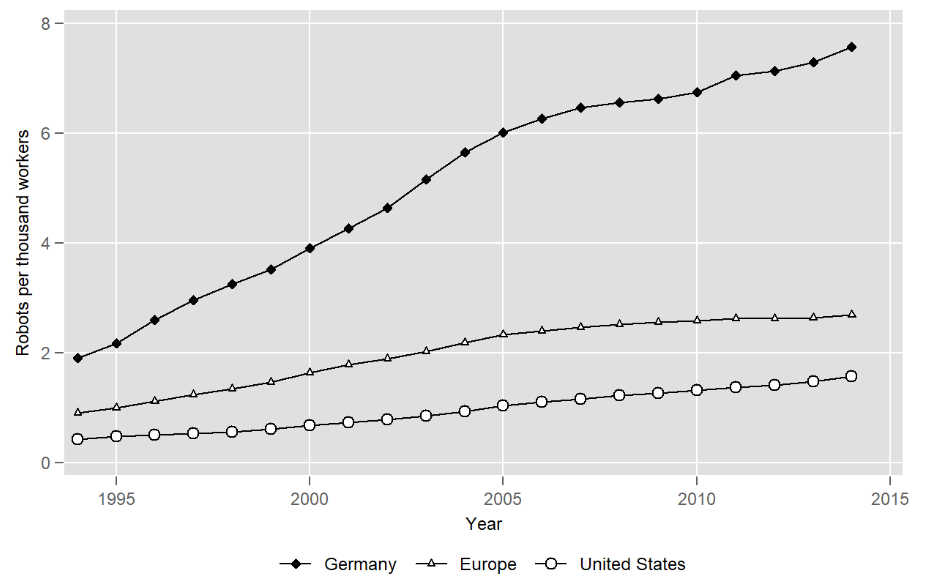
\includegraphics[width=.8\linewidth]{robots-per-workers}
    \caption{Robots per thousand workers in the industry from 1995 to 2014 \cite{dauth2017german}.}
    \label{fig:robots-per-workers}
\end{figure}

Even though robots are increasingly present in the industry, using robots to assist persons in everyday life might be more challenging. Many authors propose their use in places like schools, hospitals, and homes, including wheelchair robots, companion robots, manipulator arms for the psychically disabled and elderly populations, etc \cite{feil2005defining}. However, the dynamic and heterogeneous environment, the energy constraints and the safety are still issues in domestic use robotics.

According to Feil \cite{feil2005defining}, assistive robots are defined as ones that give support to a human user, whereas socially interactive robots are the ones that merely can interact with humans in the form of gestures, speech, etc. The intersection between these two groups is called socially assistive robots, not focusing on the interaction itself but using it as a mechanism to provide aid or assistance.

Fong \cite{fong2003survey} defines 8 traits in socially interactive robots:

\begin{itemize}
    \item Embodiment: defined as the body capabilities of the robot, the morphology, and design to deal with the ambient. Social robots design is often taken into consideration because the user must be comfortable engaging with the robot. Also, the number of sensors and actuators the robot has will expand its capabilities.
    \item Emotion: complements the embodiment in the robots by interacting in a social context. Integrating emotion in robots can create empathy and make people treat them like they treat other humans. Emotions can be displayed both as an expression, in the form of moving lips, eyebrows, eyes, and LEDs, as well as in the form of speech, in voice tone, loudness, and pitch. Body language also takes place in full-body robots.
    \item Dialogue: Creating a meaningful dialogue between two or more parties is hard even in the form of low-level dialogue. Natural language processing are still features under development and remain a great challenge to robots. Robots can also use dialog in a non-verbal way, communicating in gestures and facial display, in addition to displaying emotions.
    \item Personality: in order to correlate with users, robots must develop personality traits that will distinguish them from other robots.
    \item Human-oriented perception: to interact, robots must perceive the environment as humans do. In social situations, this includes people tracking, speech recognition, gesture recognition, and facial perception.
    \item User modeling: in addition to design and perception, they must act based on people personality, learning the user's personality to create a model on how to react.
    \item Socially situated learning: continuously learning for improving communication or acquiring new skills is essential, whether by teaching or imitation.
    \item Intentionality: lastly, humans must feel that the robot has a purpose and acts rationally. This can be achieved by demonstrating goal-directed behaviors or demonstrating attention to key objects in the scenario.
\end{itemize}

Feil goes further and defines the socially assistive robot with additional properties relative to Fong's definition:

\begin{itemize}
    \item User Populations: defines the characteristics of the user, like age, impairment, and need. He categorizes the user populations as elderly, individuals with physical impairments, individuals in convalescent care, individuals with cognitive disorders and students.
    \item Task: the author cites as task examples tutoring, physical therapy, daily life assistance, and emotional expression.
    \item Sophistication of interaction: the robot must develop beyond the emotional feature described by Fong, evolving into more complex reciprocal interactions with the user.
    \item Role of the assistive robot: the role of the assistive robot must reflect into its appearance and behavior, affecting both embodiment and personality, depending on the task and nature of the interaction.
\end{itemize}

\begin{figure}[!ht]
    \centering
    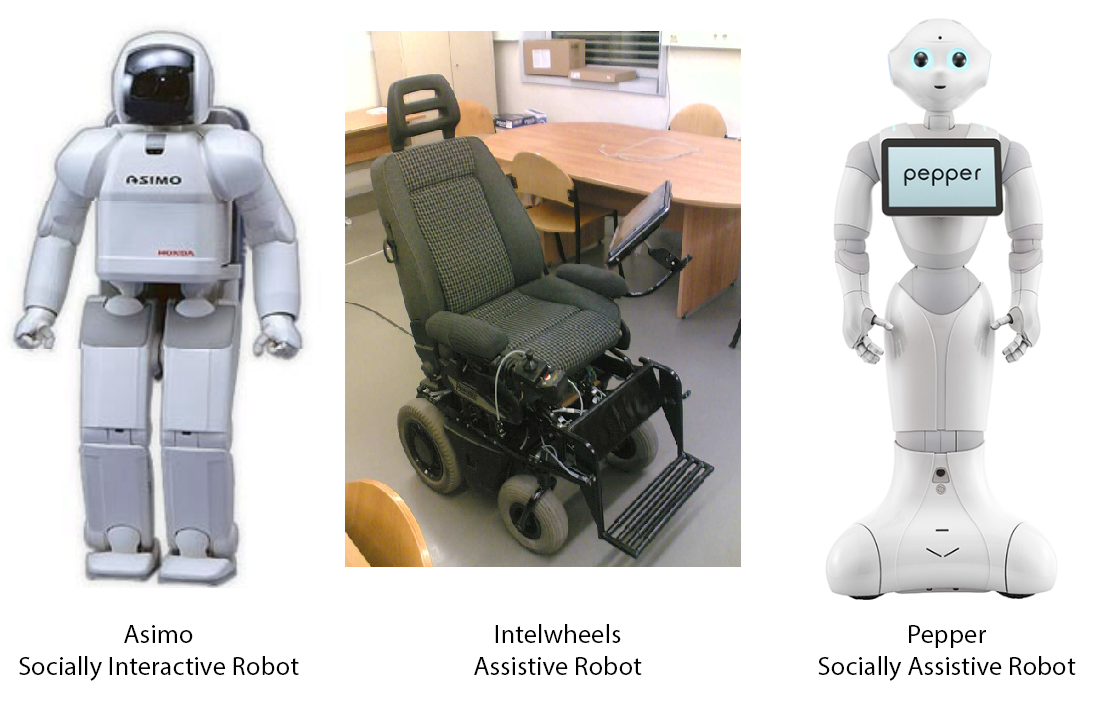
\includegraphics[width=\linewidth]{social-assistive-robots}
    \caption{Examples of Assistive and Social robots \cite{sakagami2002intelligent,braga2008intellwheels,tanaka2015pepper}.}
    \label{fig:social-assistive-robots}
\end{figure}

One of the most famous socially interactive robots developed is ASIMO, shown on the left on \prettyref{fig:social-assistive-robots}, a human-like robot developed by the Japanese company Honda in 2000. It featured a pair of legs and many features and sensors that would later be integrated into other assistive robots. Its main task was to meet visitors in the meeting room and to guide them once the manager confirms their identity. It was able to perform navigation and obstacle avoidance, respond to voice and gesture calls \cite{sakagami2002intelligent}. Even though the robot can interact with people, it does not qualify as a socially assistive robot (the first version, at the time) as defined by Feil because it couldn't fit in the user populations described. The robot was later improved to have greater grasping capabilities and a more robust sensor set.

Intelwheels is an example of an assistive robot, as seen in the middle of \prettyref{fig:social-assistive-robots}. It can assist handicapped people operating an electric wheelchair, providing not only user operation with collision avoidance but autonomous navigation. It can help elders and people with physical impairments, but the user input is one-way: it can recognize voice and facial expressions but won't interact back with the user \cite{braga2008intellwheels}.

Pepper, seen on the right on \prettyref{fig:social-assistive-robots}, was developed to fit into the category of both emotional expression and tutoring. It was aimed at the concept of the robot learning together with children using the robot's display to teach English, characterizing it as a socially assistive robot. A remote human teacher would help the process by orienting the classes. Instead of just showing the contents in the screen creating boredom, the robot engaged in playful activities with the kids, including telling them to search for a specific object in the room or repeating gestures with the robot, compelling the children to participate actively \cite{tanaka2015pepper}.

The Care-o-bot, or COB, for short, is described as a robotic home assistant aimed at helping people with mobility impairments in their daily lives. The target group includes elders, disabled, people with health conditions and with movement restraints. Its tasks include setting the table, carrying objects like books and drinks around, dealing with medication, helping the patients standing up, as well as serving as a companion to the person. The robot can also do other tasks usually performed by a nurses and doctors, like monitoring the patient with conditions in their daily routines, reminding them to take medication and calling emergency in case of incidents \cite{graf2004care}.

\begin{figure}[!ht]
    \centering
    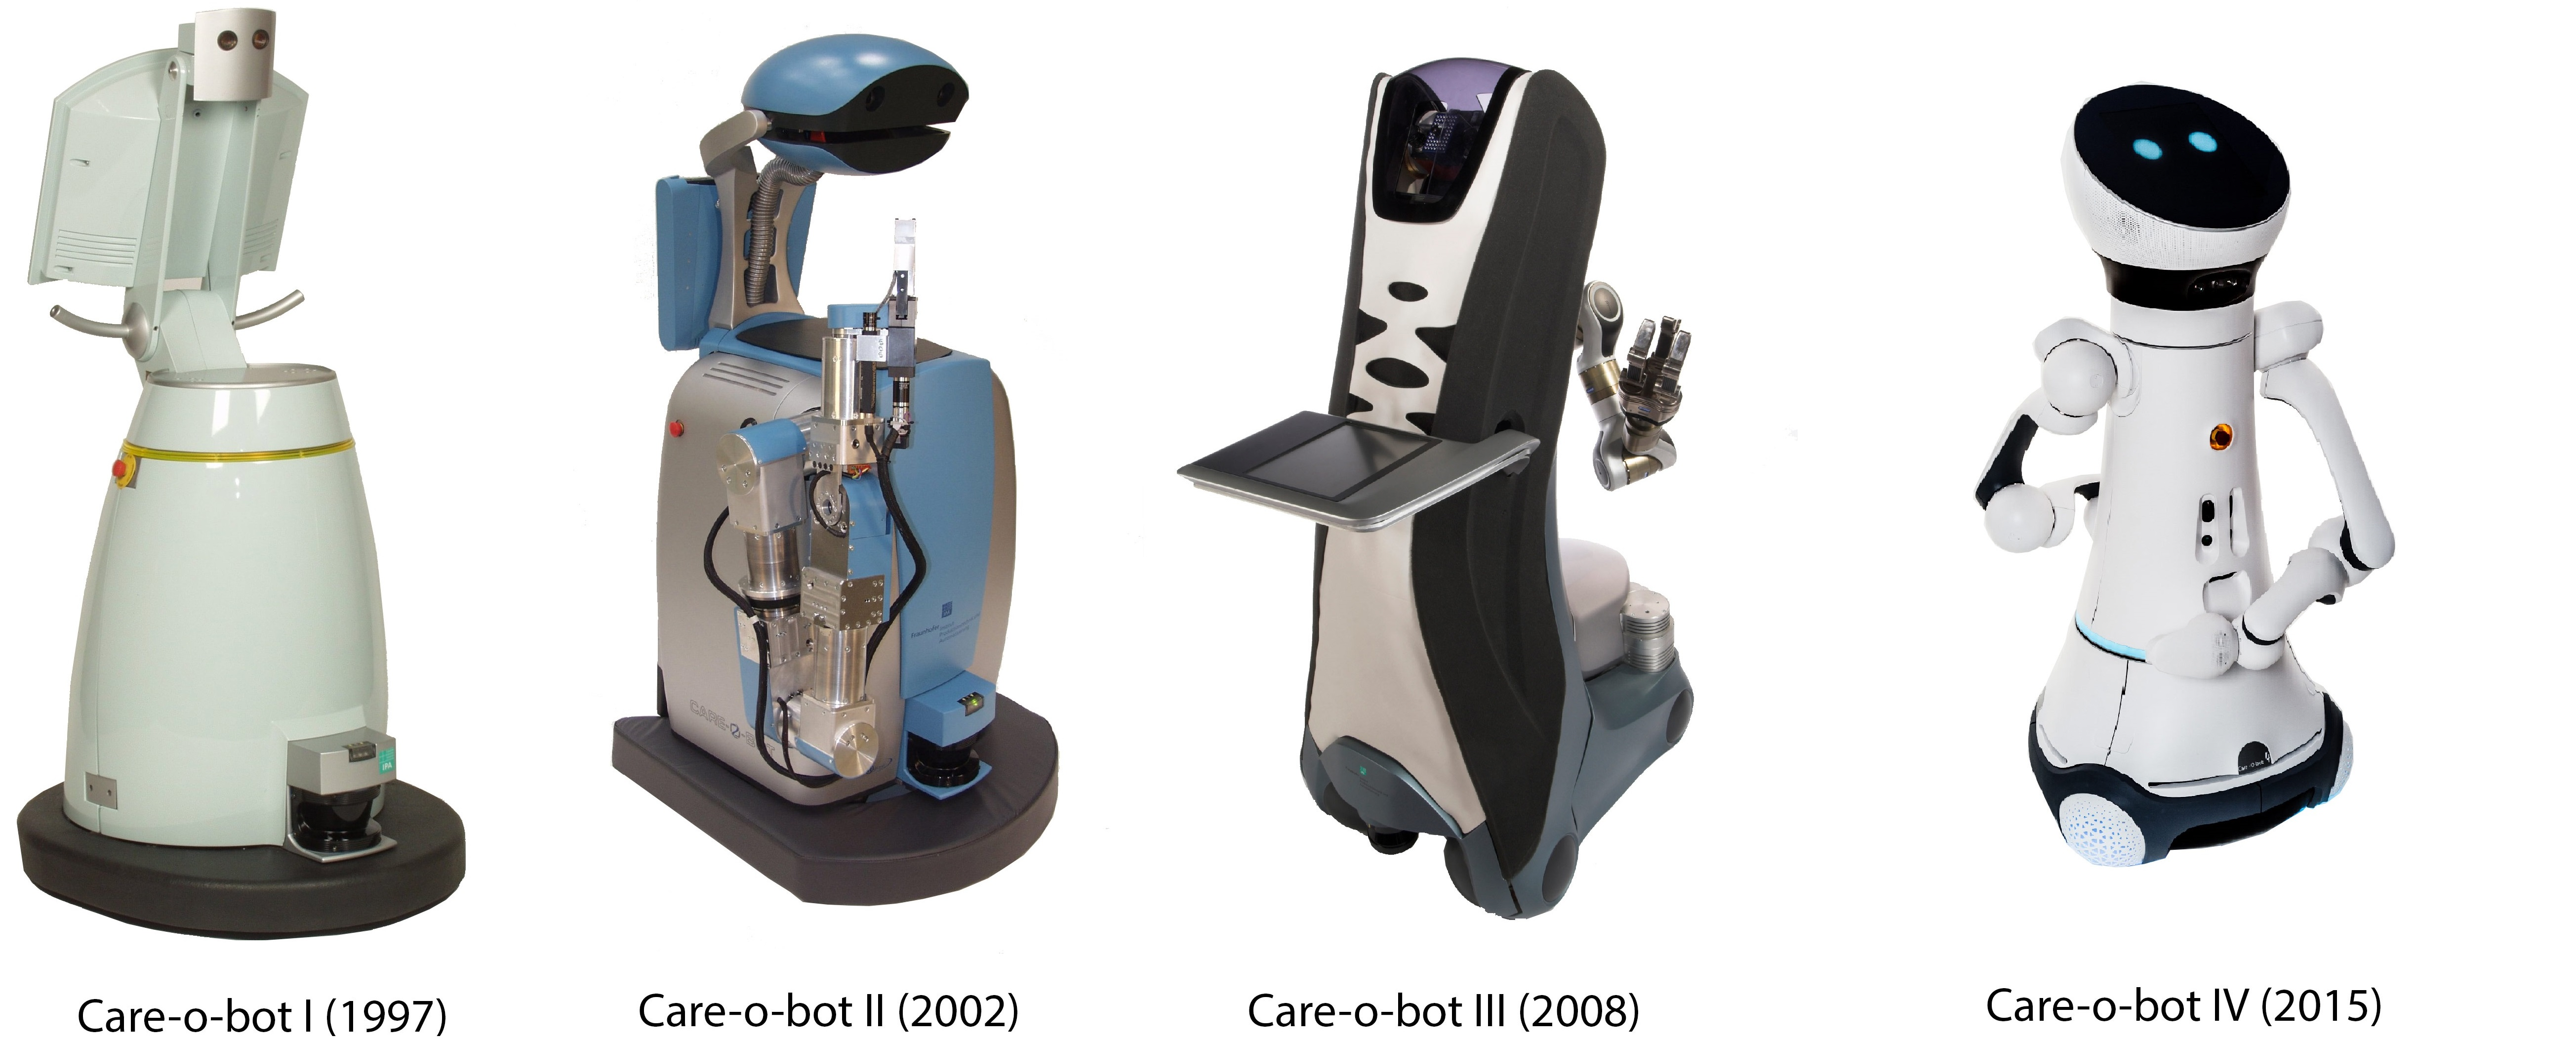
\includegraphics[width=\linewidth]{cob-evo}
    \caption{Evolution of Care-o-bot.}
    \label{fig:cob-evo}
\end{figure}

The Care-o-bot evolution throughout the years can be seen on \prettyref{fig:cob-evo}. The first prototype was built in 1997, but it didn't pack many capabilities as the technology was very limited. It was soon followed by Care-o-bot II, in 2002, equipped with a manipulator, two cameras, laser scanners, and a hand-held control panel. Version II presented great improvements in navigation, computer vision, and manipulation, but was still rudimentary, having problems in low light conditions and dynamic environments (the 3D scans could only be run once because of processing constraints) and not being recommended inexperienced users \cite{graf2004care}.

The third generation came in 2008, using a better 7DOF arm and 3 finger gripper with tactile feedback. It also became a lot more user-friendly, applying the concepts of embodiment and presenting a less bulky body with smoother surfaces and less visible mechanical parts. The robot body was divided into a working side (in the back, where the manipulator stands) and a serving side (on the front, to interact with users) \cite{graf2009robotic}.

The fourth generation was presented in 2015 and focused heavily on emotion design. It was developed to appear familiar and sociable, and avoid the uncanny valley \cite{macdorman2006subjective}, where human-like robots can cause strangeness or even fear. It featured a multi-modal user interface capable of displaying facial expressions with a minimalistic pair of eyes to display a wide range of emotions. The spherical joints in the torso and head allow more agility, the body is smaller and more efficient and more sensors and 3D cameras were installed.

One of the many challenges of assistive robots is navigating the environment. As they need to reach places in the house like the kitchen or the bedroom, they sometimes need to be aware of how to navigate through the rooms and corridors to reach the final destination. The approach described in \citeauthor{siegwart2011introduction} for this problem is running algorithms in different layers: perception, to extract meaningful data from the environment using available sensors; localization, to determine where it is relative to the environment; cognition, in order to take action given the inputs; and motion control, in order to output the right commands to the motors \cite{siegwart2011introduction}. \prettyref{fig:navigation_guidelines} shows us the guidelines to build a localization stack in a mobile robot.

\begin{figure}[!ht]
    \centering
    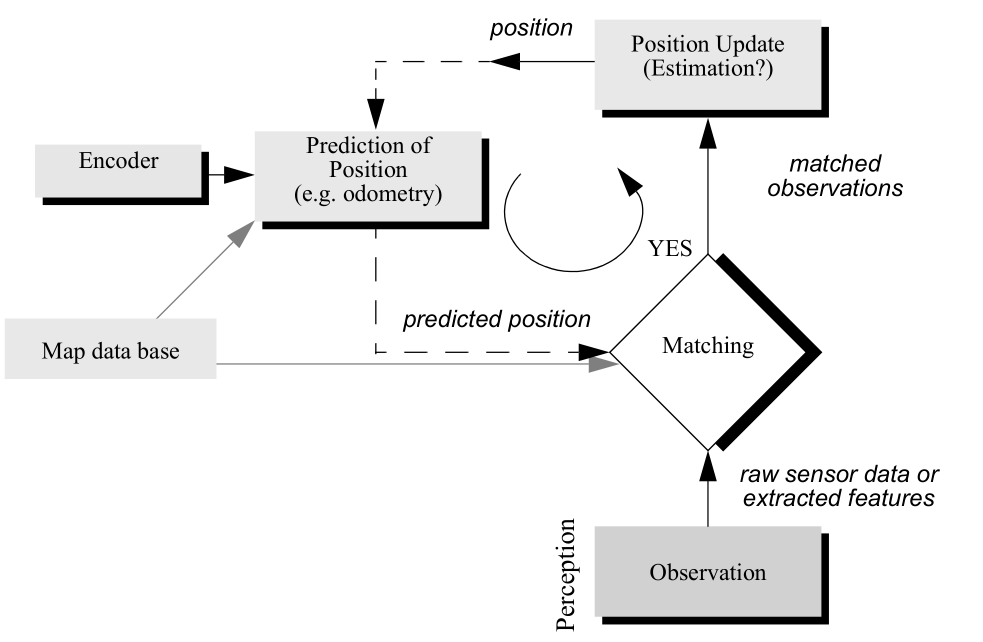
\includegraphics[width=0.8\linewidth]{navigation_guidelines}
    \caption{Localization stack flowchart \cite{siegwart2011introduction}.}
    \label{fig:navigation_guidelines}
\end{figure}

As we can see, it is necessary to sense the world. This is done through encoders in the wheels, GPS, or other forms of localization, in the form of odometry, or in observations, using 3D cameras, LIDAR, Sonar, etc. This data is fed to a matching algorithm, together with a map database, resulting in an estimated position update, that will be used as feedback for the next iteration.

However, this approach is only as accurate as the map is. Many algorithms aim to solve the mapping problem accurately, but there is no standard way of telling how accurate each algorithm is because there is no agreement on which benchmarks to use. The difficulties in comparing visual data and the absence of the ground truth impose challenges when comparing maps generated by different algorithms \cite{amigoni2007good}.

The goal of this paper is to propose a method for comparing mapping algorithms. We will test the proposed architecture against the most popular algorithms available in the open repositories, namely Gmapping, Hector, Karto and Cartographer, using data from simulated Care-o-bot. The results will be then discussed and compared against what is currently present in the literature about mapping benchmarking.

This work is structured as follows. \prettyref{chp:fundament} shows the background theory in order to understand how the tests were performed. It includes an introduction to the Robot Operating System (ROS) used in all experiments, as well as an introduction to COB hardware. \prettyref{chp:slam_mapping} explains the mapping problem into more detail and gives an introduction to how each tested algorithm works. This chapter also presents a review of the literature to come up with good metrics and an algorithm approach for comparison. A custom way of generating accurate maps is proposed and simulated using Care-o-bot. The resulting are exported into public datasets, so that they can be reused for further testing or even for different algorithms not tested in this paper.

\prettyref{chp:results} shows the results obtained using the proposed metrics and a discussion. Finally, \prettyref{chp:conclusoes} presents conclusions and discusses future work in this topic.

%state the general topic and give some background

%provide a review of the literature related to the topic

%define the terms and scope of the topic

%outline the current situation

%evaluate the current situation (advantages/ disadvantages) and identify the gap

%identify the importance of the proposed research

%state the research problem/ questions

%state the research aims and/or research objectives

%state the hypotheses

%outline the order of information in the thesis

%outline the methodology
\chapter{Background Theory}\label{chp:fundament}
%\vspace{-1.5cm}
%\noindent\rule{\columnwidth}{1.2mm}

\section{ROS}

There are many problems when developing robot applications, especially because of the complexity of those systems. As more and more functionality is added to the robot, the code base becomes fluttered with intricate dependencies and entangled libraries. ROS is not an operating system per se, but a framework that allows coders to readily develop and test solutions with modularity and code reusability in mind. It was built in an agnostic package system that allows integration with many packages available from the ROS Open-source community, a lot of them implementing support libraries and proof-of-concept algorithms, as well as core infrastructure.

The main aspects of ROS are \cite{quigley2009ros}:

\begin{itemize}
\item Peer-to-peer: even though the ROS framework relies on a master or namespace as a lookup mechanism, the communication is established between peers, avoiding unnecessary routing through slow links when the recipient is on the subnet.
\item Tools-based: instead of building an intricate framework, ROS relies on a set of tools written to perform specific tasks, including various tools for compilation, tap data stream, data plotting, configuration, documentation generation, etc. Custom tools can even be written by the user in the form of new packages.
\item Multi-lingual: since communication between nodes relies only on XML-RPC, they can be implemented in any language, either by explicitly writing the full library that interacts with the ROS Core or building a wrapper for the ROS C++ library.
\item Thin: many robots implementations have parts of the code that could be reused in another project if they weren't so entangled with all existing code. ROS proposes an architecture where the code is separated into packages that hold no dependency on ROS. All packages can be built individually using CMake, different from the traditional software paradigm where one CMake file builds the entire project.
\item Free and Open-source: ROS source code is publicly available and released under the BSD License, allowing copy and redistribution of the source code, including for commercial purposes.
\end{itemize}

The execution of ROS is separated into smaller pieces of code that do particular tasks, called nodes. Each time ROS Core is launched, a collection nodes that are required for execution are spawned: the ROS master, that provides support for the registration of all subsequent nodes, the ROS parameter server, to register parameters during execution time, and rosout, for logging purposes. Once the core is launched, every other node can be spawned.

\subsection{Packages}

In order to better build robotic systems, ROS adopts a packaged architecture, making every subsystem of the application separate from all the others. Every package can contain new nodes, libraries, configuration or even datasets.

The main advantage of this approach is making the code more organized in its own subsystems and sub-subsystems, that specialize in doing a specific task very well so that other packages can use this functionality. Packages can also be written independently of language, as long as it's supported by ROS.

\subsection{Topics}

In order for nodes to communicate, they interact by publishing messages in topics. Topics are anonymous buses where each node can publish messages following the message type standards. Each node can then subscribe to topics that are relevant to them and act upon data captured on the topic. Message can even be recorded and played back to support applications that will need the information later in time.

% TODO: refazer imagem para evitar citação
\begin{figure}[!ht]
\centering
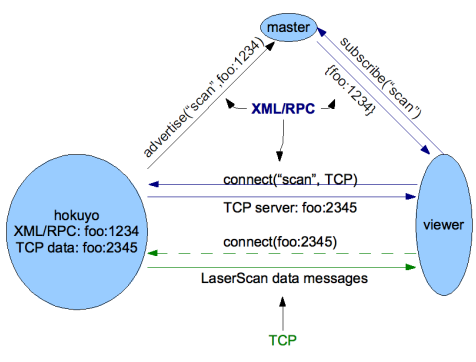
\includegraphics[width=0.5\linewidth]{rostopic}
\caption{Topic initialization \cite{rosoverview}.}
\label{fig:rostopic}
%\small{Source: ROSWiki.}
\end{figure}

The topics are implemented in the XML-RPC protocol, using a master node in order to provide name resolution. In order for a publisher to connect to a subscriber, they do the following steps \cite{rosoverview}:

\begin{enumerate}
\item Subscriber register with the master the topics it will be listening to.
\item Publisher register with the master the topics it will be publishing to.
\item Master informs the subscriber of a new publisher.
\item Subscriber requests a topic connection with the Publisher and negotiates a transport protocol.
\item Subscriber connects using the selected protocol.
\end{enumerate}

It's important to notice that, once the connection is established, the communication is maintained peer-to-peer, using former protocols like TCPROS, built over TCP/IP, and UDPROS, built over UDP. This not only provides faster communication inside the same network by not requiring the messages to be relayed through the master but also enables communication through available networks of the Internet protocol suite, including 802.11X wireless transmission.

The topic configuration also enables true agnostic packages, since the communication between them will be done using a standardized communication medium, loosely coupling the packages and making them easily maintainable. Debugging can also be done using command-line tools that wiretap this medium and display the information exchanged by nodes.

\subsection{Services}

The topic communication can be very useful in many-to-many communication but lacks support when sending messages or commands that require a response. When a reply is needed, it is a better practice to use services instead of topics. This is especially true for tasks that need a lot of computing power but only need to be executed once in a while, so instead of calculating it in every iteration, the service can be run just when requested and return data to the caller. The request is usually done in a similar way to Remote Procedure Calls (RPCs) in programming languages.

\subsection{Message types}

Since nodes need to understand each other, they talk following pre-defined message standards, and the message files themselves are packages that define the content of each message. To avoid confusion, each topic is initialized using a pre-defined message type and every node has to conform to it. Let's take a look at the message definition \texttt{geometry\_msgs/Twist.msg}, that is used in navigation to define linear and angular velocity for the joints:

\begin{lstlisting}
Vector3  linear
Vector3  angular
\end{lstlisting}

Note that the \texttt{Vector3} is not a base type message, but is another type of message defined at \texttt{geometry\_msgs/Vector3.msg}:

\begin{lstlisting}
float64 x
float64 y
float64 z
\end{lstlisting}

The variable types that cannot be expanded into other definitions are called primitive types. The primitive types are:

\begin{multicols}{3}
    \begin{itemize}
        \item \texttt{bool}
        \item \texttt{int8}
        \item \texttt{uint8}
        \item \texttt{int16}
        \item \texttt{uint16}
        \item \texttt{int32}
        \item \texttt{uint32}
        \item \texttt{int64}
        \item \texttt{uint64}
        \item \texttt{float32}
        \item \texttt{float64}
        \item \texttt{string}
        \item \texttt{time}
        \item \texttt{duration}
    \end{itemize}
\end{multicols}

Message types for services are done in a similar way, but since services support response, the message will consist of two individual messages. If we look at a standard definition found in \texttt{std\_srvs/SetBool.srv}:

\begin{lstlisting}
bool data
---
bool success
string message
\end{lstlisting}

This service is used for setting a boolean variable to \textit{true} or \textit{false}, that can be activating or deactivating an actuator. The response consists of a boolean that tells if the operation was successful and a message for better description in case of error.

\section{Transformations}

Transformations, or tfs, for short, are the way ROS deals with coordinates frames in space. As the poses for each link in the robot might change over time, it keeps track of these changes and provides tools to assist the user to do transformations with the data.

Suppose a particular robot has a reference fixed frame \texttt{/world} in the origin. The center of the robot is another frame called \texttt{base\_link}. The transformation \texttt{/world -> /base\_link} would indicate the position of the robot relative to the world.

Now, let's say the robot has a laser scanner sensor \texttt{/laser\_link} relative to \texttt{/base\_link}, as it is fixed on the robot. The laser makes a measurement and this result is relative to the laser position. Let's call the result \texttt{/result}. The result is then related to \texttt{/world} by a long chain of transformations.

\begin{verbatim}
/world -> /base_link -> /laser_link -> /result
\end{verbatim}

It can be tricky to transform the \texttt{/result} back to \texttt{/world} coordinates. The tf package gives the user an easy way of setting up a listener on the \texttt{/tf} topic that will listen to the published transforms and do the required transformations between coordinate frames, so the user can ask directly for the transform \texttt{/world -> result} instead of transforming the data himself.

\section{Simulation}

Since deploying a test robot at every code change is costly and time consuming and ROS only provides the tools to develop a robot system solution, there is a need for offline simulation of the robots, avoiding having to test every configuration on physical hardware. In these cases, it can be helpful to set up a rigid body simulation. The normal workflow for setting up a simulation is \cite{russell2004}:

% http://ode.org/slides/slide2.html
\begin{itemize}
    \item Isolating the important variables in the physical process.
    \item Model the physical system behavior using equations.
    \item Find a method to solve the equations, given the inputs and the initial state of the system.
    \item Write a computer program that can do that simulation.
    \item Simulate and benchmark the results against the physical system.
\end{itemize}

Repeating all these five steps for every physical system will lead to the best results, but can be time-consuming and difficult because all the variables involved. Since the possibilities for a robot system are often limited, physics engines or physics SDKs (source development kits) were developed to aid simulation.

While the real world has a lot of complexity, rigid body dynamics can be simplified in rigid bodies, joints, collisions, friction and springs, elements that are important to the process. The physical model can be reduced to the laws of motion, using mass, velocity, acceleration, and force as simulation variables. Since the model and the solution to these problems are well known, generalized solvers can be written that compute the simulation at each instant of time, or time steps.

Many simulators implement this generalized solvers, as well as render the 3D models to show to the user, including game engines like Unity and USARSim (based on Unreal engine), commercial solutions like Microsoft Robot Studio, Webots and MATLAB, and open-source projects like Gazebo \cite{craighead2007survey}. Since Gazebo adopts the mentality of the ROS project of being open and free, it became widely used in the community, and as a result better developed over time.

Gazebo provides ROS with a framework to simulate and benchmark the robot or even a group of robots accurately. \prettyref{fig:gazebo-sim} shows the Gazebo simulation for a supported robot \cite{koenig2004design}.

\begin{figure}[!ht]
\centering
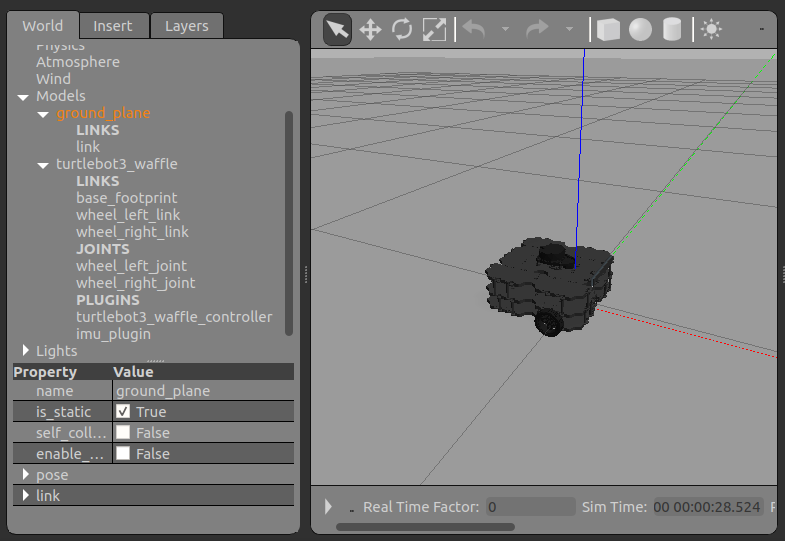
\includegraphics[width=.5\linewidth]{gazebo-sim}
\caption{Gazebo simulation suite.}
\label{fig:gazebo-sim}
\end{figure}

The Gazebo simulator offers:

\begin{itemize}
\item Dynamics simulation using multiple physics engines.
\item Advanced 3D graphics for high-quality rendering.
\item Sensors and noise, to generate reliable sensor data, compatible with real-world sensors.
\item Robot models, including ones from the community.
\end{itemize}

All the robot description is made using a URDF file or an SDF file. The URDF or Universal Robotic Description Format file is an XML file describing all elements of the robot. Even though it's called ``Universal'', it lacks some of the features like parallel linkages, friction, etc. To get around these issues, a new model called SDF or  Simulation Description Format was developed specifically for use in Gazebo, while the URDF was maintained for backward compatibility. Every time a URDF file is loaded, it is converted by Gazebo to an SDF equivalent.

\subsection{URDF}

URDF files starts describing each link of the robot and it's respective inertia. \prettyref{fig:gazebo-sim} show an example of three links of the robot Turtlebot3 Waffle \cite{turtlebot3}: \texttt{base\_footprint}, \texttt{wheel\_left\_link} and \texttt{wheel\_right\_link}. They are loaded from STL or Collada files included in the project. \prettyref{fig:gazebo-stl} show the STL renders for the robot shown on \prettyref{fig:gazebo-sim}.

\begin{figure}[!ht]
\centering
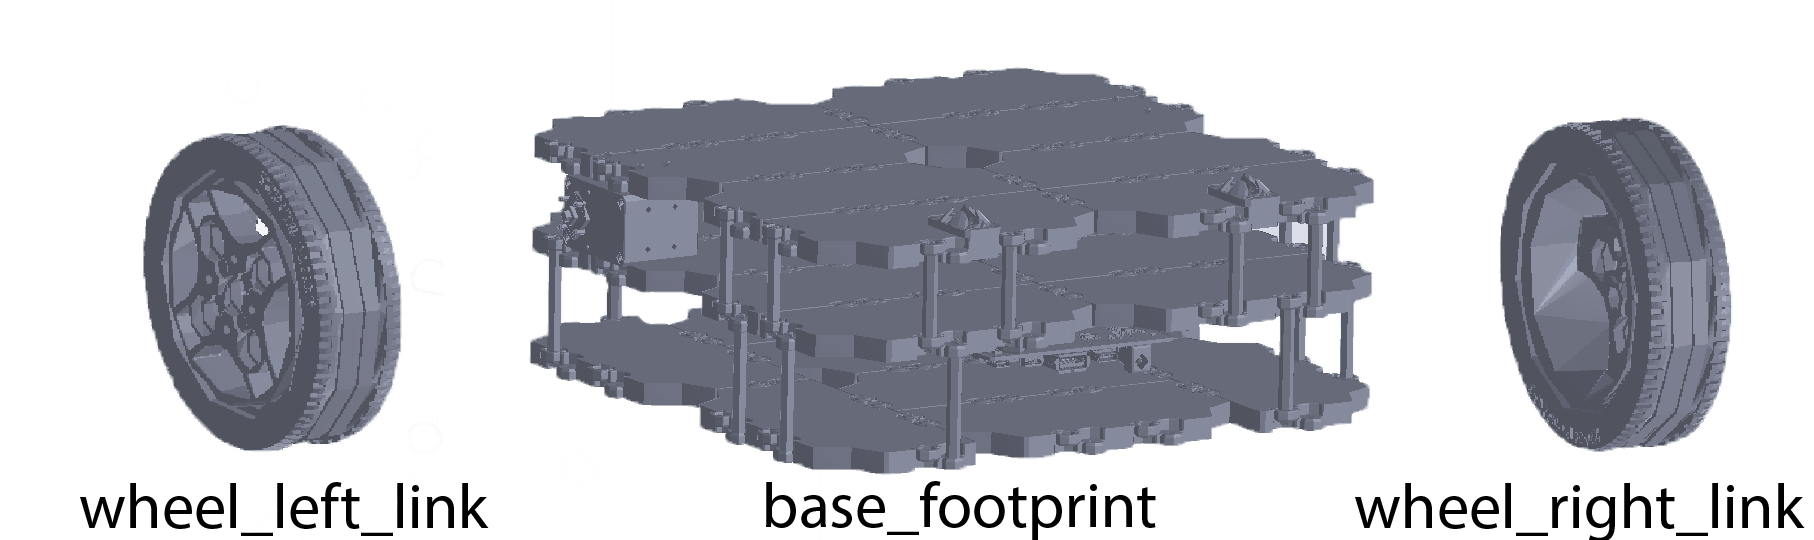
\includegraphics[width=.8\linewidth]{gazebo-stl}
\caption{STL Link files.}
\label{fig:gazebo-stl}
\end{figure}

The inertia is described by its inertial parameters, namely the mass, center of mass and moment of inertia matrix. Additionally, collision box that will aid collision testing in simulation can be specified. The user can then describe the rest of the robot, including the joints that will hold links together. Two basic joints can be seen, \texttt{wheel\_left\_joint} and \texttt{wheel\_right\_joint}, that hold all three links together. Finally, the plugins will give the robot the simulation functionality, adding IMUs, Laser Scanners, Cameras, etc.

\subsection{SDF}

The SDF is an improvement of the URDF descriptor format that supports more functionality. It not only supports all the physical descriptions shown in the URDF model but also features:

\begin{itemize}
\item World information, from lightning and gravity to complex information like magnetic fields, winds, and atmosphere (temperature and pressure).
\item Scene information, like ambient, background, sky, fog and shadows.
\item Multiple robots descriptors.
\item Choosing a physics engine.
\end{itemize}

\subsection{Physics Engines}

In order to simulate the physical conditions of the robot and the environment, Gazebo supports four different physics engines: ODE, Bullet, Simbody, and DART. At the start of each simulation, the user can select the desired physics engine changing the startup flags for the program, or configure it on the SDF file.

ODE or Open Dynamics Engine is an engine for simulating articulated rigid body structures. It features a stable integrator, meaning that numeric errors may not grow out of control. Because of that, the simulator drops physical accuracy in favor of speed, stability and robustness \cite{smith2005open}.

Bullet is a Python implementation of physics simulation for robotics, games, and visual effects that provides forward and inverse dynamics and kinematics, as well as built-in collision detection. Bullet differentiates itself by being easy to use and provides integration to machine learning frameworks like TensorFlow \cite{coumans2018}.

Simbody is a multibody simulator focused on biomedical research. It was developed to better suit simulation scenarios where engines like ODE may not converge to correct results due to its lack of fidelity. It is used for neuromuscular, prosthetic, and biomolecular simulation, as well as design and control of humanoid robots \cite{sherman2011simbody}.

DART or Dynamic Animation and Robotics Toolkit is another rigid body simulation that distinguishes itself due to its accuracy and stability. The main purpose of this simulator is to provide full access to internal kinematic and dynamic quantities \cite{lee2018dart}.

All four engines are used to tackle different problems. By varying the time step, for instance, you might obtain better results in your simulation with one of the engines. Usually, when choosing the simulation engine, the relationship between the number of iterations, error, and speed must be taken into account. Some of the simulations require greater precision, while others may require real-time performance. For a more in-depth comparison of the four engines see \cite{peters2014comparison}.

\subsection{Sensors and actuators}

Gazebo also allows simulating sensors and actuators that will interact with the world and send data back to ROS packages. Sensors can include cameras, laser scanners, contact sensors, IMU, RFID, Sonar, Magnetometer. Actuators can use the ROS control library to actuate joints. The sensors are described in the SDF or URDF files. The example below shows an example of a camera description.

\begin{lstlisting}[caption=Camera Description., language=XML]
  <gazebo reference="camera_link">
    <sensor type="camera" name="camera1">
      <update_rate>30.0</update_rate>
      <camera name="head">
        <horizontal_fov>1.3962634</horizontal_fov>
        <image>
          <width>800</width>
          <height>800</height>
          <format>R8G8B8</format>
        </image>
        ...
      </camera>
      <plugin name="camera_controller" filename="libgazebo_ros_camera.so">
        <alwaysOn>true</alwaysOn>
        <updateRate>0.0</updateRate>
        <cameraName>robot/cam1</cameraName>
        <imageTopicName>image_raw</imageTopicName>
        <cameraInfoTopicName>camera_info</cameraInfoTopicName>
        <frameName>camera_link</frameName>
        <hackBaseline>0.07</hackBaseline>
        <distortionK1>0.0</distortionK1>
        <distortionK2>0.0</distortionK2>
        <distortionK3>0.0</distortionK3>
        <distortionT1>0.0</distortionT1>
        <distortionT2>0.0</distortionT2>
      </plugin>
    </sensor>
  </gazebo>
\end{lstlisting}

The controller is loaded from a plugin called \texttt{libgazebo\_ros\_camera.so} and uses as parameters which topic the camera will correspond to and the intrinsic parameters of the lenses, update rate and sensor type, as well as the link the camera will be attached to.

There are many pre-built plugins available at Gazebo library, including Cameras (mono and stereo), Kinect, Laser Scanner, Force and IMU sensors, Differential Drive, Skid Steering Drive, as well as templates to write your own dedicated plugin.

%\section{OpenCV}

%\section{MoveIt}

%MoveIt is a ROS library aimed at simplifying motion planning for complex robots. It is the evolution of \texttt{arm\_navigation} package, designed for motion planning, trajectory generation and environment monitoring for the PR2 robot \cite{chitta2012moveit}.

%One of the main requirements of robots working closely to humans and the dynamic environment is that they can detect and avoid collisions and other obstacles efficiently. MoveIt does this by creating a probabilistic 3D model of the environment using Octomaps. This is important because physical sensors have noise and inaccuracies, and the Octree representation is also much more efficient.

%With a model in hand, MoveIt can make use one of the available planners: Open Motion Planning Library (OMPL), Stochastic Trajectory Optimization for Motion Planning (STOMP), Search-Based Planning Library (SBPL), and Covariant Hamiltonian Optimization for Motion Planning (CHOMP). Having different planners available is important because they allow different movement constraints. One trajectory might need the manipulator to be always upright, like carrying liquids, while other doesn't have this constraints. MoveIt uses a configuration wizard to generate configuration files based on the URDF or SRDF robot model, making the package robot agnostic. In the configuration, the user can specify the attributes desired for the robot.

%The Self-collisions options allow you to select the density of the Self-collision matrix. Higher densities require more computation whereas lower densities might disable valid options. Virtual joints allows you to define which joints attach the robot to the world frame. Planning groups are used to virtually separate distinct parts of the robot, that may include creating joint groups on what composes the left arm, right arm, manipulator, etc. Robot poses defines fixed poses as reference for the robot, that may include \textit{Home} or \textit{Resting} positions. The End-effectors configuration is used to further specify which of the planning groups are end effectors, that may include tools and grippers. Finally, the passive joints configuration is used to specify the joints that cannot be actuated on, and thus cannot be used for motion planning.

%There are also plugins for RVIZ visualization of the planned trajectories. They help by providing visual tools to work with the robot, examining poses and testing trajectories behavior. There are also many plugins available for Inverse Kinematics calculation, as well as wrappers to write your own solver.

\section{COB}

The Care-o-bot is a project for a mobile assistive robot that is modular, developed and maintained by Fraunhofer IPA. The COB version 4 can be seen on \prettyref{fig:cob4}. The robot was composed not only to provide researchers a reliable mobile base, but also to aid research on human-robot interaction and social behavior \cite{mci/Kittmann2015}. It is composed mainly by a mobile base, a torso, and a head.

% TODO: editar a imagem para conter descrição de partes
\begin{figure}[!ht]
\centering
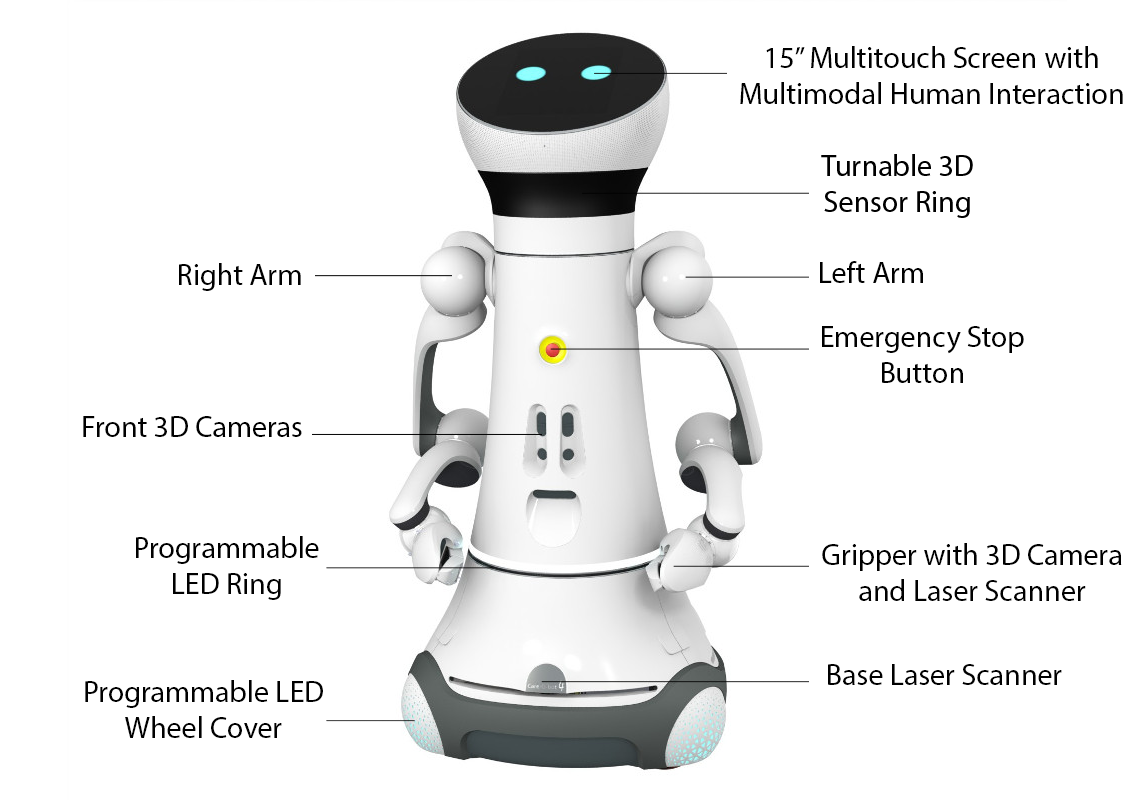
\includegraphics[width=.8\linewidth]{cob4}
\caption{COB 4 full robot with both manipulators.}
\label{fig:cob4}
\end{figure}

\subsection{Base}

The base features three steerable wheels used for moving the robot on the ground. Because the modularity, the wheels can be configured to behave using Ackermann kinematics, moving forward and backward and rotating on the vertical axis, but also Omnidirectional kinematics, allowing the robot to move in every direction. The maximum speed supported is 1,1 m/s. It is also equipped with three 2D laser scanners with 360$^{\circ}$ coverage for object detection and safety, and the battery for the robot and the control panel.

\subsection{Torso}

The torso is linked with the base, and can be configured to be fixed (the torso doesn't move), to use a Pan joint (allowing for a full rotation) or using a spherical joint (providing 3DOF). It can have two optional arms with 7DOF, each with a manipulator finger with 2DOF.

The manipulator also has a 3D camera and laser scanner for object recognition and picking, as well as LEDs for illumination. The torso also provides 3D cameras and sensors for computer vision activities that cover up the front of the robot and an LED Ring for signaling and an emergency stop.

\subsection{Arms}

The arm is composed of three SCHUNK Powerball ERB modules and one PRL+ 100 module, a rotary actuator, in the shoulder. The arm is a variation of the commercially available Schunk arm called LWA4P, which has 6 DOF and is composed of three Powerball ERB, with 2 DOF each. The last degree of freedom is provided by the PRL+, allowing one rotation around the shoulder and totaling 7 DOF. \prettyref{fig:schunk_lwa4p_extended} shows the full arm in simulation. The manipulator's finger was developed by Schunk specifically for this robot.

\begin{figure}[!ht]
    \centering
    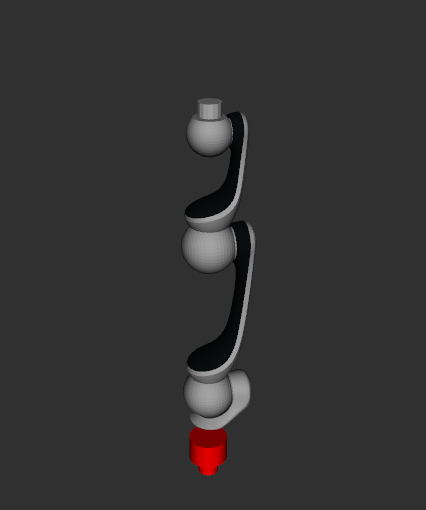
\includegraphics[width=.3\linewidth]{schunk_lwa4p_extended}
    \caption{LWA4P extended arm.}
    \label{fig:schunk_lwa4p_extended}
\end{figure}

The LWA4P arm was designed to operate at low power at battery-dependent devices and is capable of lifting a maximum payload of 6kg. Each joint in the Powerball is capable of rotating to $\pm 170^\circ$, at a maximum speed of $72^\circ /\text{s}$, and the overall repeat accuracy of the arm is $\pm 0.15 \ \text{mm}$.


\subsection{Head}

The head is linked with the torso, allowing for both a pan joint or a spherical joint, and contain the human interface to interact with the user, including the sound system, microphone, a touch screen display and optional camera for face recognition.


\subsection{Package organization}

The COB is built around ROS and combines different sets of packages for different purposes. Since the robot support different configurations (manipulators, joints, mobile bases), some packages are optional. \prettyref{fig:dependency-graph} shows the dependency graph for the first three layers of packages. Notice that the arrangement is quite intricate even showing only the packages written exclusively for COB (not showing other ROS packages used on COB).

\begin{figure}[!ht]
\centering
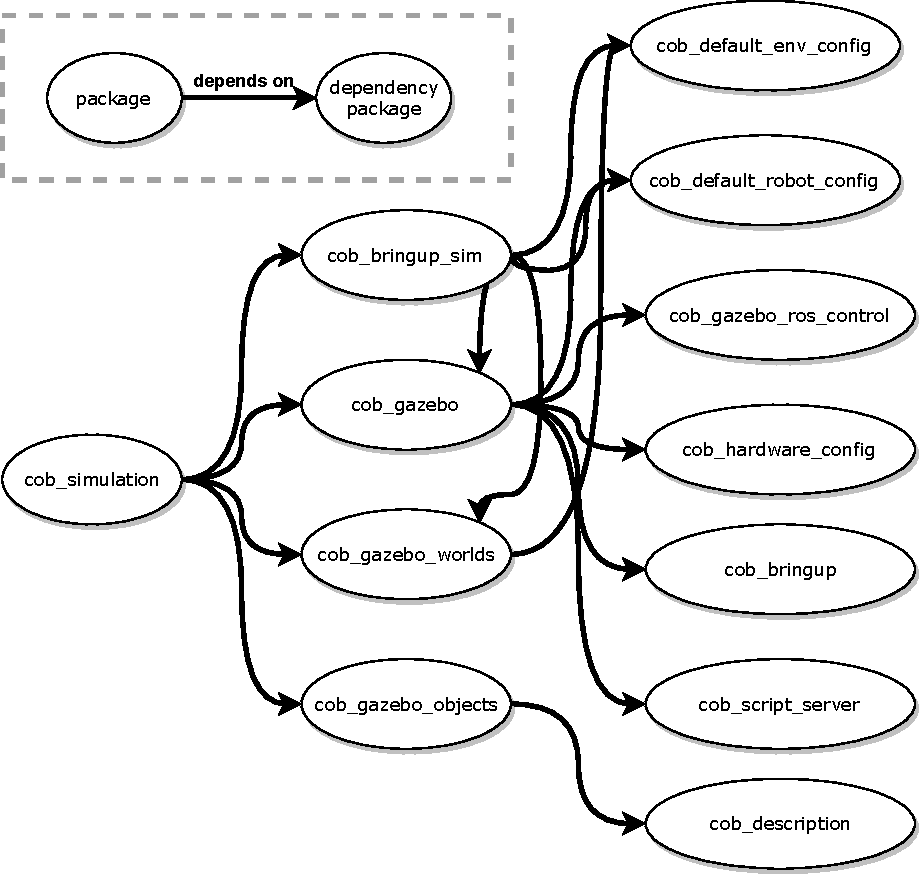
\includegraphics[width=.7\linewidth]{dependency-graph}
\caption{Dependency graph of \texttt{cob\_simulation} with depth 3.}
\label{fig:dependency-graph}
\end{figure}


The COB core consist of the following packages and its dependencies:

\begin{itemize}
\item \texttt{cob\_msgs}: Robot-specific Messages, representing state information like battery status, etc.
\item \texttt{cob\_srvs}: Robot-specific Services.
\item \texttt{cob\_description}: Robot URDF models for different COB configurations (only base, base with fixed torso, base with actuated torso, etc).
\item \texttt{cob\_bringup}: machine configuration, including all scripts and dependencies required to run COB, both in simulation and real hardware.
\end{itemize}

COB also features high-level capabilities, some of them being:

\begin{itemize}
\item \texttt{cob\_command\_tools}: high-level utilities command tools, including API for commonly used movements, control dashboard, teleoperation and status monitoring.
\item \texttt{cob\_driver}: plugins interfacing motors, LEDs, sound system, cameras, batteries and even the facial expressions for the robot, and providing their data in the form of topics and services.
\item \texttt{cob\_navigation}: provides tools for robot navigation, including creation of maps, navigation with/without collision avoidance and navigation in dynamic environments.
\item \texttt{cob\_object\_perception}, \texttt{cob\_people\_perception}, \texttt{cob\_environment\_perception}: computer vision libraries used for perception of the environment.
\item \texttt{cob\_manipulation}: manipulator related package, including inverse kinematics, arm motion planning and collision avoidance.
\end{itemize}

\subsection{Basic API}

Most of the capabilities of COB are exposed in the form of topics and services, forming a higher level API and sparing the user from interacting with low-level sensors and actuators.

The actuators move the three wheels on the base. Since the base kinematics is already calculated by the node, you only need to supply a \texttt{geometry\_msgs/Twist} type message with linear and angular velocities and the drivers will take care of the rest. The topic names can be seen on \prettyref{tab:baseapi}.

\begin{table}[!ht]
\caption{Base command API.} \label{tab:baseapi}
\renewcommand*{\arraystretch}{1.1}
\resizebox{\textwidth}{!}{
\begin{tabular}{c|c|c}
Topic Name & Message Type & Information \\
\hline
\makecell{\texttt{/base/twist\_mux} \\ \texttt{/command\_navigation}} & \texttt{geometry\_msgs/Twist} & Velocity topics related to navigation \\ \hline
\makecell{\texttt{/base/twist\_mux} \\ \texttt{/command\_safe}} & \texttt{geometry\_msgs/Twist} & \makecell{Velocity topics related to teleoperation \\ with collision checking and smoothing} \\ \hline
\makecell{\texttt{/base/twist\_controller} \\ \texttt{/command}} & \texttt{geometry\_msgs/Twist} & \makecell{Low level Velocity topics \\ for control purposes} \\ \hline
\end{tabular}
}
\end{table}

Since the torso and the head only have one joint, they receive a set of points forming a trajectory to follow, given by the \texttt{control\_msgs/FollowJointTrajectory} service message type. This service returns if the robot was able to perform the trajectory, as well as the error in the path. The structure can be seen on \prettyref{tab:headapi}.

\begin{table}[!ht]
\caption{Torso and head command API.} \label{tab:headapi}
\renewcommand*{\arraystretch}{1.1}
\resizebox{\textwidth}{!}{
\begin{tabular}{c|c|c}
Topic Name & Message Type & Information \\
\hline
\makecell{\texttt{/torso/joint\_trajectory\_controller} \\ \texttt{/follow\_joint\_trajectory}} & \texttt{control\_msgs/FollowJointTrajectory} & Trajectory to move the torso \\ \hline
\makecell{\texttt{/head/joint\_trajectory\_controller} \\ \texttt{/follow\_joint\_trajectory}} & \texttt{control\_msgs/FollowJointTrajectory} & Trajectory to move the head \\ \hline
\end{tabular}
}
\end{table}

The Arms, the Grippers and the sensor ring are similar to the torso and head, as they act as a service and receive the same message type. Their API is shown on \prettyref{tab:armapi}.

\begin{table}[!ht]
\caption{Arms and grippers command API.} \label{tab:armapi}
\renewcommand*{\arraystretch}{1.1}
\resizebox{\textwidth}{!}{
\begin{tabular}{c|c|c}
Topic Name & Message Type & Information \\
\hline
\makecell{\texttt{/arm\_left/joint\_trajectory\_controller} \\ \texttt{/follow\_joint\_trajectory}} & \texttt{control\_msgs/FollowJointTrajectory} & Trajectory to move the left arm \\ \hline
\makecell{\texttt{/gripper\_left} \\ \texttt{/joint\_trajectory\_controller} \\ \texttt{/follow\_joint\_trajectory}} & \texttt{control\_msgs/FollowJointTrajectory} & Trajectory to move the left gripper \\ \hline
\makecell{\texttt{/arm\_right/joint\_trajectory\_controller} \\ \texttt{/follow\_joint\_trajectory}} & \texttt{control\_msgs/FollowJointTrajectory} & Trajectory to move the right arm \\ \hline
\makecell{\texttt{/gripper\_right} \\ \texttt{/joint\_trajectory\_controller} \\ \texttt{/follow\_joint\_trajectory}} & \texttt{control\_msgs/FollowJointTrajectory} & Trajectory to move the right gripper \\ \hline
\makecell{\texttt{/sensorring} \\ \texttt{/joint\_trajectory\_controller} \\ \texttt{/follow\_joint\_trajectory}} & \texttt{control\_msgs/FollowJointTrajectory} & Trajectory to move the sensor ring ring\\ \hline
\end{tabular}
}
\end{table}

For the sensors, there are three lasers scans that cover the entire circumference of the robot, shown on \prettyref{tab:laserapi}. Even though they are separate entities, there are nodes that transform the three different measurements into a single one for easier use later on.

\begin{table}[!ht]
\caption{Laser Scan API.} \label{tab:laserapi}
\centering
\renewcommand*{\arraystretch}{1.1}
\begin{tabular}{c|c|c}
Topic Name & Message Type & Information \\
\hline
\texttt{/base\_laser\_front/scan} & \texttt{sensor\_msgs/LaserScan} & Front laser scan \\ \hline
\texttt{/base\_laser\_left/scan} & \texttt{sensor\_msgs/LaserScan} & Left laser scan \\ \hline
\texttt{/base\_laser\_right/scan} & \texttt{sensor\_msgs/LaserScan} & Right laser scan \\ \hline
\texttt{/scan\_unified} & \texttt{sensor\_msgs/LaserScan} & Unified laser scan \\ \hline
\end{tabular}
\end{table}

There are also cameras in the torso, head and in the sensor ring that collect both raw images and a Point Cloud representation that includes the distance of each point to the focal point of the camera. Their respective topics can be seen on \prettyref{tab:cameraapi}.

\begin{table}[!ht]
\caption{Cameras API.} \label{tab:cameraapi}
\renewcommand*{\arraystretch}{1.1}
\resizebox{\textwidth}{!}{
\begin{tabular}{c|c|c}
Topic Name & Message Type & Information \\
\hline
\texttt{/torso\_cam3d\_left/rgb/image\_raw} & \texttt{sensor\_msgs/Image} & \makecell{Color image of the \\ left torso camera} \\ \hline
\texttt{/torso\_cam3d\_left/depth\_registered/points} & \texttt{sensor\_msgs/PointCloud2} & \makecell{Depth data from \\ torso left camera} \\ \hline % left camera
\texttt{/torso\_cam3d\_right/rgb/image\_raw} & \texttt{sensor\_msgs/Image} & \makecell{Color image of the \\ right torso camera} \\ \hline
\texttt{/torso\_cam3d\_right/depth\_registered/points} & \texttt{sensor\_msgs/PointCloud2} & \makecell{Depth data from \\ torso right camera} \\ \hline % right camera
\texttt{/torso\_cam3d\_right/rgb/image\_raw} & \texttt{sensor\_msgs/Image} & \makecell{Color image of the \\ down torso camera} \\ \hline
\texttt{/torso\_cam3d\_down/depth\_registered/points} & \texttt{sensor\_msgs/PointCloud2} & \makecell{Depth data from \\ torso down camera} \\ \hline % down camera
\texttt{/sensorring\_cam3d\_front/depth/points} & \texttt{sensor\_msgs/PointCloud2} & \makecell{Depth data from \\ sensor ring camera} \\ \hline
\texttt{/sensorring\_cam3d\_back/rgb/image\_raw} & \texttt{sensor\_msgs/Image} & \makecell{Color image of the \\ back sensor ring camera} \\ \hline
\texttt{/torso\_cam3d\_down/depth\_registered/points} & \texttt{sensor\_msgs/PointCloud2} & \makecell{Depth data from \\ back sensor ring camera} \\ \hline % sensor ring back camera
\texttt{/head\_cam3d/rgb/image\_raw} & \texttt{sensor\_msgs/Image} & \makecell{Color image of the \\ head camera} \\ \hline % head camera
\end{tabular}
}
\end{table}

Finally, there are also other miscellaneous topics to control the lights and text-to-speak output and publish robot information, shown on \prettyref{tab:miscapi}.

\begin{table}[!ht]
\caption{Miscellaneous API.} \label{tab:miscapi}
\centering
\renewcommand*{\arraystretch}{1.1}
\resizebox{\textwidth}{!}{
\begin{tabular}{c|c|c}
Topic Name & Message Type & Information \\
\hline
\texttt{/joy} & \texttt{sensor\_msgs/Joy} & Input commands of joystick \\ \hline
\texttt{/sound/say} & \texttt{cob\_sound/Say} & Text for text-to-speak output \\ \hline
\texttt{/light\_base/set\_light} & \texttt{cob\_light/SetLightMode} & Command for base lights \\ \hline
\texttt{/light\_torso/set\_light} & \texttt{cob\_light/SetLightMode} & Command for torso lights \\ \hline
\texttt{/light\_torso/set\_light} & \texttt{cob\_light/SetLightMode} & Command for torso lights \\ \hline
\texttt{/emergency\_stop\_state} & \texttt{cob\_msgs/EmergencyStopState} & \makecell{Laser and button \\ stop information.} \\ \hline
\texttt{/power\_state} & \texttt{cob\_msgs/PowerState} & \makecell{Battery information.} \\ \hline
\end{tabular}
}
\end{table}
\chapter{SLAM}\label{chp:slam_mapping}

One of the first challenges in indoor navigation for assistive robots is actually finding where they are. Robot localization is fundamental to not only know where you need to go, but rather find a path there that avoids the obstacles.

Mapping is an essential tool in this matter, and it comprises the areas of \textit{concurrent mapping} and \textit{localization problem}. In themselves, both problems are relatively easy and well understood: mapping an environment knowing the localization and localizing the robot having the map in hands are simple tasks. However, the combination of those two problems is hard to solve \cite{thrun2000real}.

Many SLAM (Simultaneous Localization and
Map Building) algorithms emerged to try and solve these problems, using different approaches and range of sensors to do the task. Some even evolved fusing data from different sensors to provide higher precision. They often rely on assumptions about the system nature. Most of the algorithms assume that the noise can be modeled  as a gaussian. Others might assume that the movement is linear and apply Kalman Filters to predict the current state.

\section{Sensors}

\subsection{Laser Scanners}

The laser scanner is one of the most simple ways to capture data about the environment. They work by sending beams of light in a direction and measuring the time it takes for the light to travel back and forth between the object and the sensor. As you want information to be gathered on more than a single point, the scanner can rotate a mirror or even the whole sensor to gather measurements from all directions, as shown on \prettyref{fig:sick_s300_diagram}. There are two main ways of measuring the object distance: time of flight and Phase-Shift \cite{amann2001laser}.

\begin{figure}
     \centering
     \subfloat[][]{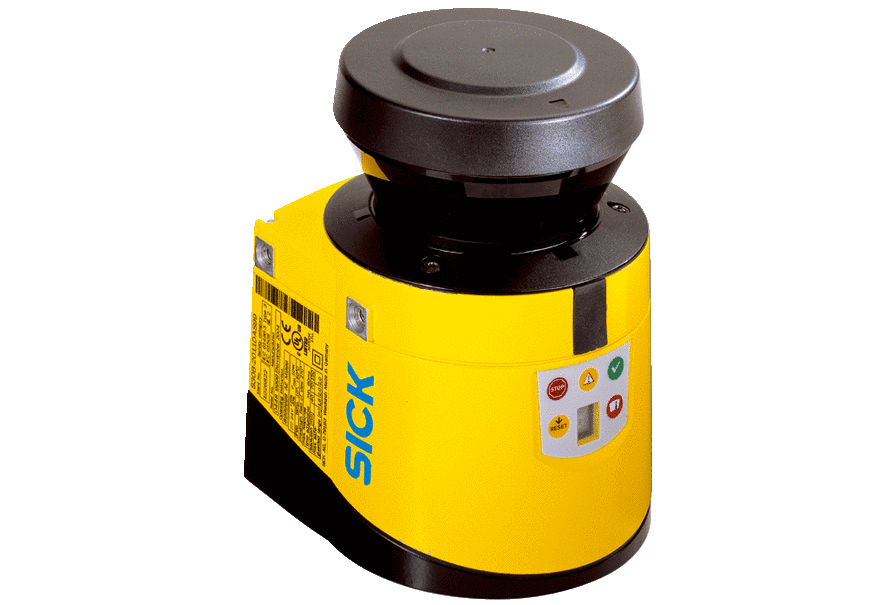
\includegraphics[width=80mm]{sick_s300}}
     \subfloat[][]{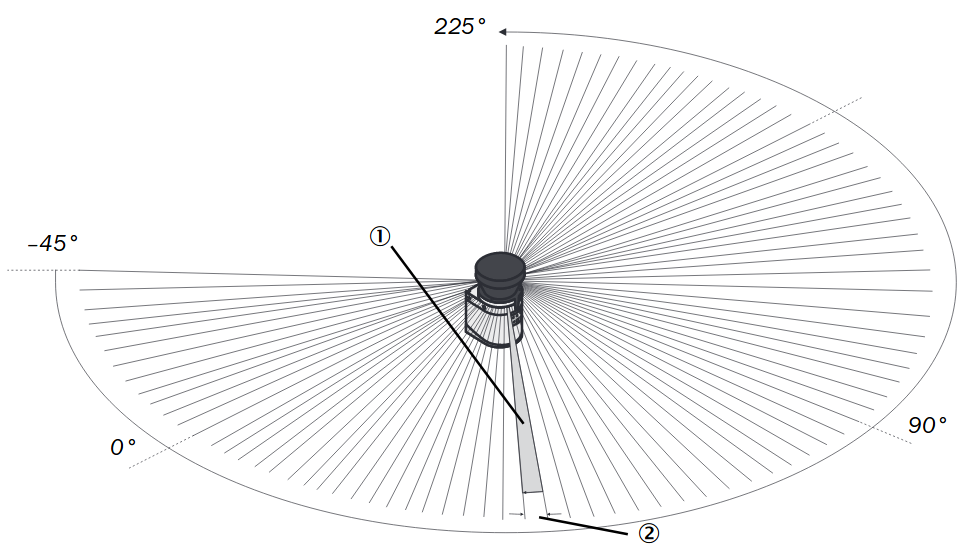
\includegraphics[width=80mm]{sick_s300_diagram}\label{fig:sick_s300_diagram}}
     \caption{SICK S300 Laser Scanner \cite{sicks300}.}
     \label{fig:sick_s300}
\end{figure}

In the time of flight measurement, a stopwatch is started when the beam of light is emitted. Since the speed of light is well known, the calculations are very straight forward, as shown on \prettyref{eq:d}. This form of measurement depends heavily on the quality of construction, as the usual sources of inaccuracy are noise (electronics, radiation in the room), timing (stopwatch precision, pulse detection), and minimal changes in each measurement can lead to big errors in the final result. Averaging and Filtering also take a big role in providing reliable data.

\begin{equation} \label{eq:d}
D = \frac{c \cdot t}{2}
\end{equation}

The second way of calculating the distance is by using phase-shift techniques, assuming there will be a difference in phase between the beam of light emitted and received. This varies according to the frequency and time traveled according to the equation $\phi = \omega \cdot t$, where $\phi$ is the phase-shift, $t$ the time traveled and $\omega$ the angular frequency of the wave. Isolating $t$ and substituting in \prettyref{eq:d}, we can derive the \prettyref{eq:d2} that dictates the distance based on frequency. This technique also requires more complex signal processing structures like a heterodyne for good for measurements.

\begin{equation} \label{eq:d2}
D = \frac{1}{2} \frac{c \cdot \phi}{\omega} = \frac{1}{4 \pi} \frac{c \cdot \phi}{f}
\end{equation}

%\subsection{3D cameras}

%Even though it is possible to recreate a 3D model of the environment using LIDAR laser scanners, discussed on the last subsection, those sensors coast thousands of dollars and are not very suited for robotics. Fortunately, it is possible to replace those sensors with 3D cameras capable of registering depth based on image processing techniques.

\section{Localizing the robot}

\subsection{Wheel Odometry}

Wheel odometry is one of the most simple ways to determine the position of the robot based on the starting point. Considering a flat surface, simply taking the turns made by each wheel and the steering actions, it is possible to estimate the path the robot took by applying the forward kinematics of the base.

\begin{figure}
    \centering
    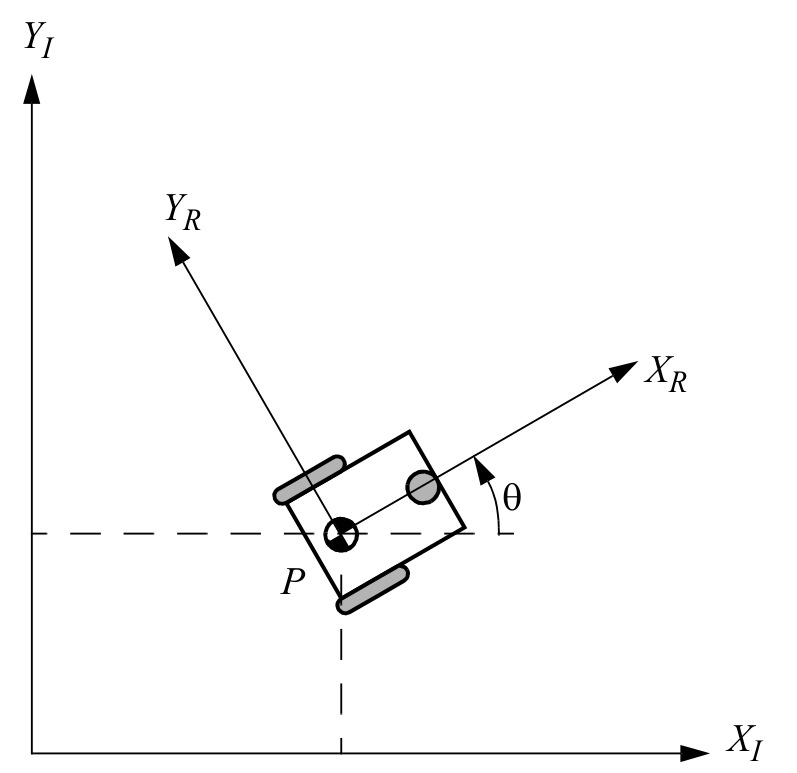
\includegraphics[width=0.4\linewidth]{fk}
    \caption{Forward Kinematics of Mobile Robot \cite{thrun2005probabilistic}.}
    \label{fig:fk}
\end{figure}

Considering the robot from \prettyref{fig:fk}, the position according to the global coordinate system can be represented by $\xi_I = [x, y, \theta]$, as well as the velocity $\dot{\xi} = [\dot{x}, \dot{y}, \dot{\theta}]$. The velocity model for the robot coordinate system can be written as:

\begin{equation}
\dot{\xi_R} = 
\begin{bmatrix}
\cos \theta && \sin \theta && 0 \\
- \sin \theta  && \cos \theta && 0 \\
0 && 0 && 1
\end{bmatrix}
\cdot 
\begin{bmatrix}
\dot{x} \\
\dot{y} \\
\dot{\theta}
\end{bmatrix}
=
R(\theta) \cdot \dot{\xi_I}
\end{equation}

It is easy to calculate the inverse problem using the inverse matrix $R^-1(\theta)$, converting back from the robot coordinate frame to the global frame. The only missing parameter is how the wheel kinematics translate to the $\dot{\xi_R}$ robot velocity, and that will depend on the robot wheel arrangement (wheel type, number of wheels, radius) and the robot dimensions.

The main disadvantages of wheel odometry are that the robot is limited to flat terrain, and even then slippery and small changes to forward kinematics (i.e. radius of the wheel changes slightly) can accumulate error over time, as there is not suitable way to correct the error without other sources of information.

\subsection{Laser Odometry}

Laser odometry bases itself on Laser Scanner data to localize the robot. Instead of using odometry to watch how the robot moves in the environment, it uses the collected data to see how the environment moves in relation to the robot.

One approach to this calculation would be taking two consecutive laser scanners and comparing them. It is assumed that the environment is mostly static so not much should change from one set of data to the other. The transformation that minimizes the distance between points from the two sets is then considered to be movement of the robot in that time slot.

As the small movements are integrated over time, this approach has the same flaws as wheel odometry, with error accumulating over time. However, the robot can improve the accuracy by keeping a laser scanner measurement history and repeating the minimization between many poses. It can also take advantage if it revisits a point in the past where the measurement was more accurate, as it can use data from that measurement for comparison.

\section{The localization and mapping problem}

The localization process can be expressed mathematically as follows \cite{thrun2005probabilistic}. Since all the measurements are discrete and supposing we want the localization of the robot through time, it can be represented as:

\begin{equation}\label{eq:x}
    X_t = \{x_0, x_1, \dots, x_t\} 
\end{equation}

The map can also be represented by a variable M as follows. Notice also that the map is considered to be time invariant in this case, and only depends on $n$ which is the number of features in the world.

\begin{equation}
    M = \{m_0, m_1, \dots, m_{n - 1}\}
\end{equation}

In order to do that, it is necessary to have some idea on how the robot is interacting with the world, how it is moving or the sensors readings. This can be for instance the measurements of robot odometry (wheel or laser odometry) or IMU data. The set of this measurements is defined as:

\begin{equation}
    U_t = \{u_0, u_1, \dots, u_t\}
\end{equation}

To also build the map, the robot will need the set of observations of the world, that can come as measurements from 3D cameras, LIDAR, SONAR, etc. This set of measurements is defined as:

\begin{equation}
    Z_t = \{z_0, z_1, \dots z_t\}
\end{equation}

Since every measurement in the robot is noise, the position can only be represented as a \textit{belief}, where the belief is the probability that the robot is in a position given the set of inputs and measurements. This can be represented as:

\begin{equation}
    bel(x_t, M) = p(x_t, M | u_{1, t}, z_{1,t})
\end{equation}

There are three main approaches to solve this problem, Extended Kalman Filters, Particle Filters and Graph based.

\subsection{Representing the map}

One of the concerns of mobile robots is how to build a map that is compatible with the environment and represents obstacles properly. While in some applications it is possible to have a pre-compiled map from the environment using the floor plan as a reference, those can be obsolete when dealing with highly dynamic environments or when objects get in the way. Even in static environments, there is a need to compensate for faulty or noise sensors, errors in localization, and the pre-compiled maps should only be used as complementary information. One of the techniques that emerged to solve these problems, and later was adopted as the core of many SLAM algorithms, is the Occupancy Grid \cite{elfes1989using} representation.

The Occupancy Grid is form of representing obstacles in 2D or 3D where each cell on the grid stores the probabilistic information of that area. This especially useful because it provides a comprehensive way to fuse sensor data, based on probability, instead of out-of-the-box algorithms that require fine tuning to work.

\begin{figure}[!ht]
    \centering
    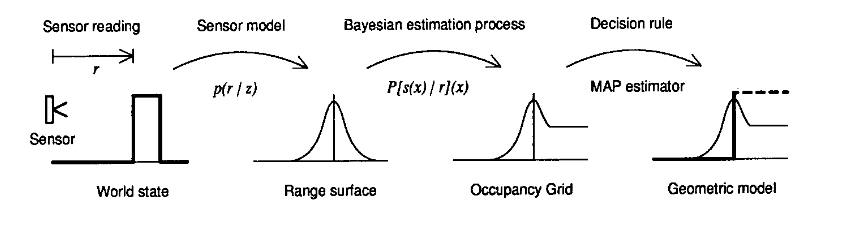
\includegraphics[width=.9\linewidth]{grid_steps}
    \caption{Steps when building an occupancy grid \cite{elfes1989using}.}
    \label{fig:grid_steps}
\end{figure}

According to \prettyref{fig:grid_steps}, the first step when building a sensor grid is to get the sensor reading. The next step is build a sensor model $p(r|z)$. Then, the Bayesian estimation is applied, based on all the observations before and current observations, to update the map. Finally, the world model is obtained using an estimator such as \textit{maximum a posteriori} (MAP). All those steps are done by the SLAM algorithms using different techniques, but even with default tuning those algorithms are good enough to work on most scenarios.

Naturally, the obstacle cell is labeled as occupied, with probability 1. All the cell until this one are labeled as empty, with probability 0. The unknown cells are labeled with unknown, with probability 0.5.

\begin{figure}[!ht]
    \centering
    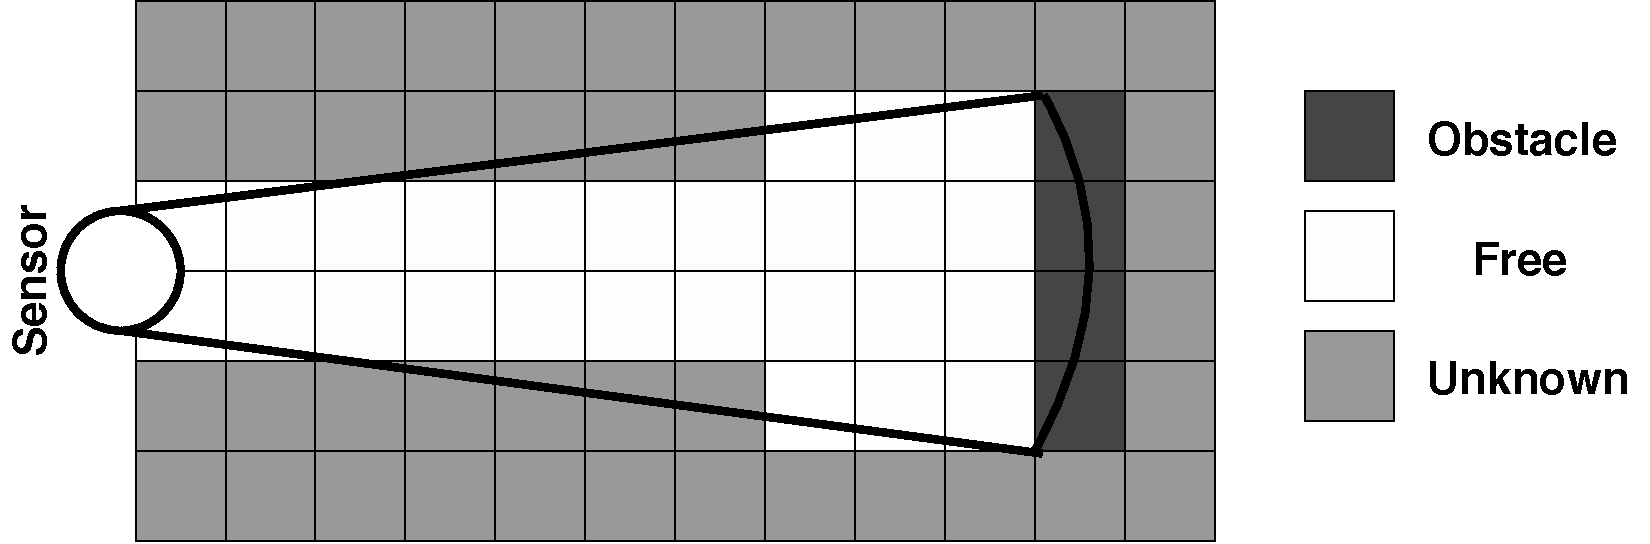
\includegraphics[width=.9\linewidth]{occupancy_grid}
    \caption{Occupancy grid for a single sensor.}
    \label{fig:occupancy_grid}
\end{figure}

The process is iterative and, as measurements from different points of view and different sensors grow, the maps become more and more complete, as shown on \prettyref{fig:occupancy_grid_algorithm}. The data fusion can also be done in different manners, but is commonly done using Kalman filters or Extended Kalman filters.

\begin{figure}[!ht]
    \centering
    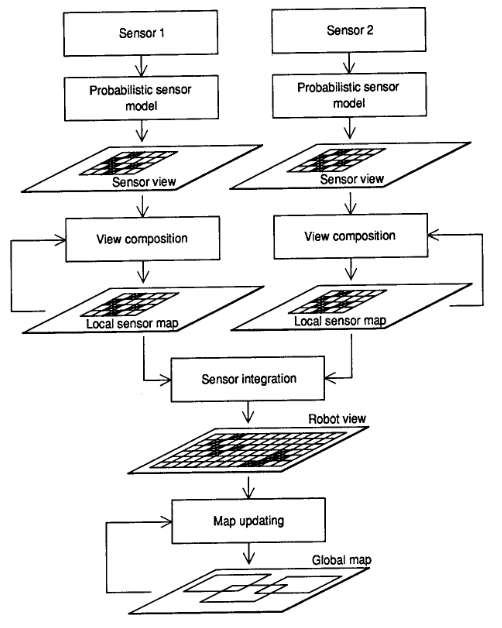
\includegraphics[width=.9\linewidth]{occupancy_grid_algorithm}
    \caption{Occupancy grid algorithm for multiple sensors.}
    \label{fig:occupancy_grid_algorithm}
\end{figure}

\section{ROS Slam Algorithms}

\subsection{Gmapping}

Gmapping is by far the most famous SLAM algorithm in robotics for a number of reasons. It was originally proposed by \citeauthor{doucet2000rao} in 2000 as way of using Particle filters algorithms with Rao-Blackwellized techniques. The main advantage of their approach is dealing with non-gaussian distributions that Kalman filters cannot deal with without rough linearization, as well as being less complex to implement.

\citeauthor{grisetti2007improved} in 2007 proposed improvements to \citeauthor{doucet2000rao} techniques in order to reduce complexity and make the resampling step better. It works by first reducing the amount of particles needed to be stored combining the current observation and odometry information, contrary to previous approaches where only odometry was used, reducing the estimation error and getting a more refined map. The second technique is using an adaptative resampling technique, meaning that resampling only has to be done when needed, reducing the problem with particle depletion, when only few particles are in high-probability areas and a lot of particles represent pretty old and unreliable information.

\subsection{Hector}

Hector SLAM first emerged in 2013 to solve the very specific problem of mapping in uneven terrains. It was aimed to be used in rescue robots that have to be robust enough to drive through ramps and obstacles and still be able to estimate the trajectory and map without reliable odometry information. Instead of trying to filter data to only include useful data, Hector pose estimation completely drops odometry data in favor of laser scanner data, and instead uses a fast LIDAR data scan-matching to estimate odometry. In order to estimate 6DOF, when moving in uneven terrain, the algorithm will also need a IMU device, and optional localization devices  like GPS, barometers and accelerometers. All the data is then fused using an Extended Kalman Filter (EKF), and not including odometry information is a simple way to exclude all errors caused by wheel spin, drift or slippery ground \cite{kohlbrecher2011flexible}.

\subsection{Karto}

Karto is a graph-based SLAM algorithm developed by Karto Robotics and made open-source in 2010. Graph-based SLAM, proposed initially by \citeauthor{lu1997globally}, works by organizing the robot pose information into a graph and then optimizing it to make it more consistent and minimize an error function. While the construction of the graph is heavily sensor dependant, optimizing the graph is computational expensive and the reason why Graph-based SLAM took so long to become popular \cite{grisetti2010tutorial}.

The graph is constructed representing every pose for the robot as a node in the graph. Every robot movement is then represented as an edge in the graph that connect the poses, this data usually being the odometry information. If the robot comes back to a known position, the algorithm does the loop closure and connects the graph to a previously known node. Since the odometry is not reliable, it has to be corrected using the laser scanner measurements. The scan observation in both poses are then matched to calculate the virtual transformation that should map one measurement optimally to the other. Let $z_{i,j}$ be the odometry information between poses $i$ and $j$ and $\hat{z_{i,j}}$ be the expect measurement, the error can be calculated simply subtracting one from the other.

\begin{equation}
    e_{i,j}(x_i, x_j) = z_{i,j} - \hat{z_{i,j}}
\end{equation}

The goal is to ultimately build a function $F(x)$ using the log-likelihood strategy:

\begin{equation}
    F(x) = \sum_{\langle i, j \rangle \ \in \ \mathcal{C}} e_{i,j}^T \Omega_{i,j} e_{i,j}
\end{equation}

so that it can be minimized by the optimization algorithm for $x^*$. In order words, what is the optimal path that minimizes the observed error, given the distribution $\Omega$ and the measurements $z$ and $\hat{z}$.

\begin{equation}
    x^* = \text{argmin}_x \ F(x)
\end{equation}

The optimization is the main problem when dealing with graph-based SLAM, and many different approaches exist to solve this problem. Karto uses Sparse Pose Adjustment, that takes advantage of the sparsity on the large matrices required to solve the problem \cite{konolige2010efficient}.

\subsection{Cartographer}

Cartographer is a fairly recent SLAM technique developed by Google. The concept behind the algorithm can be seen on \prettyref{fig:cartographer}. The main idea is separating the matters into two different problems: local SLAM and Global SLAM. The main objective is not having to deal with big maps or representations while mapping a new area. Instead, a submap is created for the local area and updated every new scan. Every scan is also tested against the submap using a Ceres-based scan matcher, to do pose optimization.

The idea of having submaps is that it is only build using a few scans, meaning that the estimate should be very close to reality. As the submaps grow larger, so does the error, meaning that every few scans a new submap is started. The Global SLAM thread will then have a collection of submaps to compute the whole map running loop closure \cite{cartographer2016google}.

\begin{figure}[!ht]
    \centering
    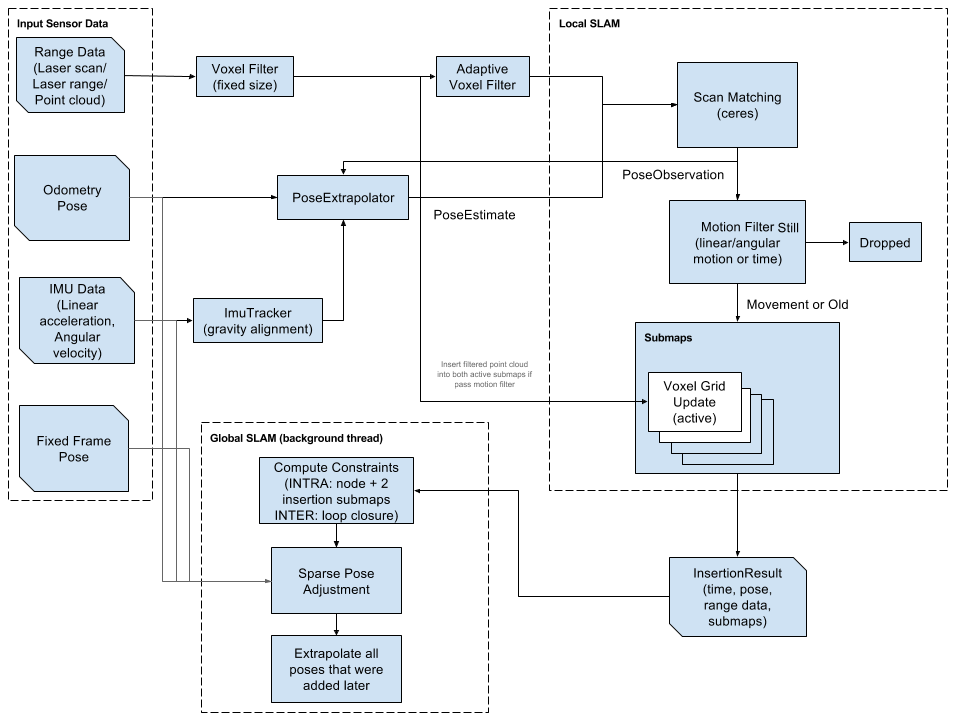
\includegraphics[width=0.6\linewidth]{cartographer}
    \caption{High-level System overview of Cartographer.}
    \label{fig:cartographer}
\end{figure}

\section{Evaluating SLAM Performance}

There is a lot of debate on how to evaluate SLAM performance. Since there are plenty of algorithms using different techniques, each one of the having their own set of parameters, there is a need to inspect them and tell which one does better in each scenario. A lot of this evaluation is done visually, assisted by a human that tells whether the occupancy grid is adequate considering the building floor plans. But as SLAM algorithms gets more precise, it is difficult to draw conclusions just from the appearance itself. Plus, there is the problem of not having the floor plants for publicly available datasets, making it harder to compare between methods \cite{kummerle2009measuring}.

According to \citeauthor{amigoni2007good}, the following issues have to be addressed when comparing SLAM:

\begin{itemize}
    \item The dataset must be pubicly available, examples being MIT Killian Court or the Intel Research Lab dataset.
    \item All algorithm parameters have to be indicated.
    \item The behavior for algorithm have to tested with different parameters in order to evaluate robustness.
    \item The dataset must include a closed-loop test, where the robot runs around an environment and comes back to the same place, to test against algorithm divergence.
    \item The ground truth must be used to evaluate results when available.
    \item Bad mapping results must be shown.
\end{itemize}

The most natural way of analyzing the poses is the squared error from the pose estimates against the ground truth. By calculating the distance from one to another and adding over time, we can get a good metric for the pose error. Considering the $x_i$ as the pose calculated by the SLAM and $x_i^*$ the ground truth pose, we can derive the \prettyref{eq:error_squared} for the squared error.

\begin{equation}\label{eq:error_squared}
\epsilon(x) = \frac{1}{N} \sum_{i}^N (x_i - x_i^*)^2
\end{equation}

\citeauthor{kummerle2009measuring} proposes a framework to analyze mapping accuracy, but uses visual inspection in order to estimate the relations between the robot poses and the environment. The estimation is then compared to the SLAM results and the final metric is the "deformation energy" required to transform the mapped result into ground truth. In other words, each of the $N_c$ displacements $\delta_{i,j}$ is compared against the ground truth $\delta_{i,j}^*$ using the \prettyref{eq:displacement}, for a set of  $(i,j)$ pairs.

\begin{equation}\label{eq:displacement}
    \epsilon(\delta) = \frac{1}{N_c} \sum_{i, j} trans(\delta_{i,j} \ominus \delta_{i,j}^*)^2 + rot(\delta_{i,j} \ominus \delta_{i,j}^*)^2
\end{equation}

 The displacement $\delta_{i, j}$ is simply calculated by the the transformation between a local measurement between two known poses, from pose $x_i$ to pose $x_j$, as described in \prettyref{eq:x}. Evaluating the displacement instead of the global position is great because it makes the evaluation resilient to small errors at the start of mapping that would impact every subsequent global position, even when the mapping in the next steps is done correctly. Since the ground-truth displacement is not available, this implementation relies on the fact that the relation between two poses can be calculated using the laser scanner, each pose later evaluated by a human. It also relies on a good enough initial guess, also human assisted. The authors also assume just evaluating the poses without evaluating the resulting map is enough for SLAM benchmarking. While this hold true for most cases, it is still very hard to infer global performance, as global displacements (large enough distance between $i$ and $j$) also carry the problem of accumulating human error, as each measurement is supervised.
 
 \citeauthor{santos2013evaluation} propose a more in-depth comparison with the publicly available SLAM algorithms that run on ROS. The authors ran both noise-free simulation and real-life experiments with the scenarios and analyzed the error metric between the ground-truth map and the generated map, also evaluating the CPU usage for each algorithm. The authors however didn't provide extensive information on how the maps were aligned, very important since the fit has to be optimal in order to do adequate comparison.
 
 \section{Proposed Evaluation techniques}
 
 In order to better evaluate the algorithms, general guidelines will be respected:
 
 \begin{itemize}
     \item Algorithms available in ROS will be used, to ensure every algorithm is publicly available for testing.
     \item Different maps will be tested to ensure no algorithm is favored. In each run, each algorithm will receive the same working data in the form as ROS bags.
     \item The scenario will be simulated in a map carefully generated using a public tool, to make sure everyone can generate the same testing data. Even though there are differences between simulation and reality, it is the only way to acquire real ground-truth data for the environment.
     \item Maps will test the ability for the algorithm to do accurate mapping, accurate localization and loop-closure. Different measurement techniques will be used to ensure all this three aspects of each map are analysed.
 \end{itemize}
 
The articles discussed already give us a good indication on what to aim for in a comparison algorithm. The first comparison method chosen is the one described in \cite{kummerle2009measuring}, as it best describe local error in the form of displacements when analyzing the trajectory of the robot. Since the ground-truth data is now available and doesn't have to be inferred by a human operator, the process can be done autonomously and we can ensure the data perfectly matches the environment.

The second comparison method chosen is the one demonstrated in \cite{santos2013evaluation}, only that now the approach for lining up the maps and calculating the error metric will be fully described. This approach will help analyzing the quality of the generated map regarding the placement of walls and objects, including their orientation and the amount of noise.

The third metric will focus on analyzing the modeled empty space of each algorithm, to see if the area of the generated room matches the area of the map. This is useful in combination with the last algorithm to see how good is the scale on each map.

\section{Building an accurate map}

It is very important to build accurate maps for SLAM testing, as the resulting map has to be compared against the ground truth and any inaccuracies might lead to different results. For that, a map generation script has been written to generate accurate Gazebo SDF descriptions of the desired map.

To generate a map, we begin with the model we want for the map to be generated with a small image file. As an example, \prettyref{fig:map_generation} is 200x200 pixels. We then draw black pixels that will represent the walls in the generated map. We run the script to generate the map and the result will be something like \prettyref{fig:gazebo_generation}.

\begin{figure}[!ht]
     \centering
     \subfloat[][]{
\includegraphics[width=.45\linewidth]{map_generation}\label{fig:map_generation}}
     \hfill
     \subfloat[][]{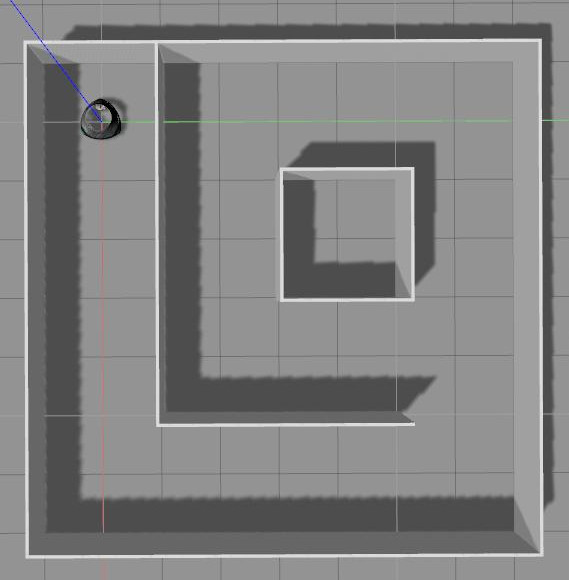
\includegraphics[width=.45\linewidth]{gazebo_generation}\label{fig:gazebo_generation}}
     \caption{Scripted map generation for Gazebo.}
     \label{fig:map_generation_script}
\end{figure}

The main body for the SDF world description can be seen on Listing~\ref{lst:sdf_header}. The only information that has to be filled is the \texttt{\{robot\_start\_pose\}} that will define where the robot will start within the map. The \texttt{\{content\}} tag will then contain a list of walls that compose the test scenario.

\begin{lstlisting}[caption={SDF Header.},label={lst:sdf_header},language=XML]
<?xml version='1.0'?>
<sdf version='1.6'>
    <model name='autogenerated'>
    <pose frame=''>{robot_start_pose} 0 0 0 0</pose>
    
    {content}
    
    <static>1</static>
    </model>
</sdf>
\end{lstlisting} \label{lst:1}

Each wall can be represented by the XML shown in Listing~\ref{lst:sdf_body}. Each will have a unique link name guaranteed by an increasing integer called \texttt{\{link\_number\}}. The \texttt{\{size\}} and \texttt{\{height\}} are the dimensions of the wall. Finally, the \texttt{\{position\}} and \texttt{\{orientation\}} represent the location of the wall center in the world, relative to \texttt{\{robot\_start\_pose\}}.

\begin{lstlisting}[caption={SDF for a single wall.},label={lst:sdf_body},language=XML]
        <link name='Wall_{link_number}'>
            <collision name='Wall_{link_number}_Collision'>
            <geometry>
                <box>
                <size>{size} {height}</size>
                </box>
            </geometry>
            <pose frame=''>0 0 0 0 0 0</pose>
            </collision>
            <visual name='Wall_{link_number}_Visual'>
            <pose frame=''>0 0 0 0 0 0</pose>
            <geometry>
                <box>
                <size>{size} {height}</size>
                </box>
            </geometry>
            <material>
                <script>
                <uri>file://media/materials/scripts/gazebo.material</uri>
                <name>Gazebo/Grey</name>
                </script>
                <ambient>1 1 1 1</ambient>
            </material>
            </visual>
            <pose frame=''>{position} 0 0 0 {orientation}</pose>
        </link>
\end{lstlisting}

\section{Selecting maps}\label{sec:selecting_maps}

The maps have to be selected to be include the scenarios encountered in real life. We selected three maps shown in \prettyref{fig:generated_maps}.

The first map can be seen on \figurename~\ref{subfig:test3}. It is meant to test the loop closure capabilities of each algorithm, since the robot will have to do the full circle and come back to the same point, and then connect the two pathways.

The second map seen on \figurename~\ref{subfig:test2}. It is a more complex version of the first map, and will test the capability of the algorithm to maintain scale between different rooms, as the corridor on the left and the loop on the right are separated by walls.

The third map sown on \figurename~\ref{subfig:test3} will test how the localization performs without revisiting positions, as the robot goes to the center of the loop without previous information and then comes back.

\begin{figure}[!ht]
     \centering
     \subfloat[][]{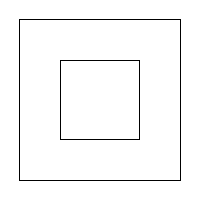
\includegraphics[width=.3\linewidth]{test1}\label{subfig:test1}}
     \subfloat[][]{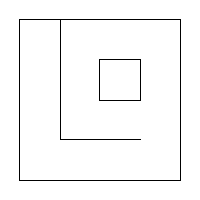
\includegraphics[width=.3\linewidth]{test2}\label{subfig:test2}}
     \subfloat[][]{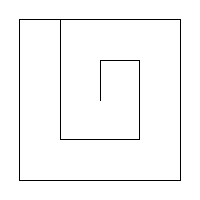
\includegraphics[width=.3\linewidth]{test3}\label{subfig:test3}}
     \caption{Selected maps for testing.}
     \label{fig:generated_maps}
\end{figure}

\section{Setting up the SLAM Algorithms}\label{sec:slam}

The following configuration was used for each of the tested algorithms. If no specified, the default configuration is being used. Cartographer is the only algorithm that also require a Lua file for configuration. All algorithms require the same hardware setup: a source of odometry, in this case a transfomation from the robot fixed frame \texttt{odom\_combined} to \texttt{base\_link} and the laser scanner data, represented by the topic \texttt{scan\_unified} that combines the data from all three lasers scanners on the robot base.

Every output then publishes the calculated map into the \texttt{map} topic and a correction of odometry using a transformation from \texttt{map} to \texttt{odom\_combined}. This transformation is a small displacement between the two frames to account for errors in the odometry for the robot that accumulate over time and can be reduced by taking the pose corrected by SLAM.

\subsection{Gmapping}

To start Gmapping, we call the launch file shown in Listing~\ref{lst:gmapping}. It starts the node \texttt{slam\_gmapping} from package \texttt{gmapping}. The laser scan topic is remapped to match the robot topic name with the \texttt{remap} tag and the odometry frame is provided as \texttt{odom\_combined}. The \texttt{map\_update\_interval} and number of particles are kept in the default configuration. The \texttt{xmin}, \texttt{xmax}, \texttt{ymin} and \texttt{ymax} are the initial size of the resulting map in meters and won't impact the results, as they are automatically increased if the map needs to be bigger. The \texttt{delta} is the map resolution and is kept at the default value of 0.05 pixels/meter.

\begin{lstlisting}[caption={Gmapping launch file.},label={lst:gmapping},language=XML]
<launch>
  <node pkg="gmapping" type="slam_gmapping" name="slam_mapping" output="screen">
    <remap from="scan" to="scan_unified"/>
    <param name="odom_frame" type="string" value="odom_combined"/>
    <param name="map_update_interval" value="5.0"/>
    <param name="particles" value="30"/>
    <param name="xmin" value="-8"/>
    <param name="ymin" value="-8"/>
    <param name="xmax" value="8"/>
    <param name="ymax" value="8"/>
    <param name="delta" value="0.05"/> <!-- map_resolution -->
  </node>
</launch>
\end{lstlisting}

\subsection{Hector}

The Hector mapping node is started using the launch script in Listing~\ref{lst:hector}, starting the node \texttt{hector\_mapping} from package \texttt{hector\_mapping}. We first remap the laser scan to the right topic and use the adequate frame names for the map, base link and odometry link. The \texttt{pub\_map\_odom\_transform} is set to True to publish the transform from \texttt{map} to \texttt{odom\_combined}. The \texttt{laser\_min\_dist} is set to the minimum value registered for the COB laser scanners.

\begin{lstlisting}[caption={Hector launch file.},label={lst:hector},language=XML]
<launch>
  <node pkg="hector_mapping" type="hector_mapping" name="slam_mapping"    output="screen">
    <remap from="scan" to="scan_unified"/>
    <param name="map_frame" value="map" />
    <param name="base_frame" value="base_link" />
    <param name="odom_frame" value="odom_combined" />
    <param name="pub_map_odom_transform" value="true"/>
    <param name="laser_min_dist" value="0.05">
  </node>
</launch>
\end{lstlisting}

\subsection{Karto}

The Karto mapping node is started using the launch script in Listing~\ref{lst:karto}, starting the node \texttt{slam\_karto} from package \texttt{slam\_karto}. We only have to set the the scan and odometry frames. The \texttt{map\_update\_interval} and \texttt{resolution} are set to the same values as Gmapping.

\begin{lstlisting}[caption={Karto launch file.},label={lst:karto},language=XML]
<launch>
  <node pkg="slam_karto" type="slam_karto" name="slam_mapping" output="screen">
    <remap from="scan" to="scan_unified"/>
    <param name="odom_frame" value="odom_combined"/>
    <param name="map_update_interval" value="5"/>
    <param name="resolution" value="0.05"/>
  </node>
</launch>
\end{lstlisting}

\subsection{Cartographer}

The Cartographer node requires a lot of configuration compared to the other SLAM algorithms. Two separate nodes have to be called at start, as seen in Listing~\ref{lst:cartographer}: the \texttt{cartographer\_node} and \texttt{cartographer\_occupancy\_grid\_node}, both from package \texttt{cartographer\_ros}.

The main Cartographer node does all the sub-map generation, and takes as parameters a Lua file with the algorithm configuration, shown in Listing~\ref{lst:cartographer_lua}. The configuration file uses all the default parameters available in Cartographer example files (in file \texttt{backpack\_2d.lua}), with the exception that the IMU was disabled, since COB doesn't have one. The frames were set accordingly and the option \texttt{provide\_odom\_frame} was set to true to get the map to odometry transform during execution. The laser scan was changed from multi echo laser scan to laser scan.

The second node is the occupancy grid node, that reads data from the sub-map list and republishes into the \texttt{/map} topic as a standard Occupancy Grid message from ROS. The resolution is also set to 0.05 pixels/meter.

\begin{lstlisting}[caption={Cartographer launch file.},label={lst:cartographer},language=XML]
<launch>
  <!-- Arguments -->
  <arg name="configuration_basename" default="cartographer.lua"/>

  <!-- cartographer_node -->
  <node pkg="cartographer_ros" type="cartographer_node" name="slam_mapping"
        args="-configuration_directory $(find cob_bringup_sim)/launch
              -configuration_basename $(arg configuration_basename)"
        output="screen">
    <remap from="scan" to="scan_unified" />
  </node>

  <!-- cartographer_occupancy_grid_node -->
  <node pkg="cartographer_ros" type="cartographer_occupancy_grid_node"
        name="cartographer_occupancy_grid_node"
        args="-resolution 0.05" />
</launch>
\end{lstlisting}

\begin{lstlisting}[caption={Cartographer Lua configuration.},label={lst:cartographer_lua},language=Python]
include "map_builder.lua"
include "trajectory_builder.lua"

options = {
  map_builder = MAP_BUILDER,
  trajectory_builder = TRAJECTORY_BUILDER,
  map_frame = "map",
  tracking_frame = "base_link",
  published_frame = "base_link",
  odom_frame = "odom_combined",
  provide_odom_frame = true,
  use_odometry = false,
  num_laser_scans = 1,
  num_multi_echo_laser_scans = 0,
  num_subdivisions_per_laser_scan = 10,
  num_point_clouds = 0,
  lookup_transform_timeout_sec = 0.2,
  submap_publish_period_sec = 0.3,
  pose_publish_period_sec = 5e-3,
  trajectory_publish_period_sec = 30e-3,
  rangefinder_sampling_ratio = 1.,
  odometry_sampling_ratio = 1.,
  imu_sampling_ratio = 1.,
}

MAP_BUILDER.use_trajectory_builder_2d = true
TRAJECTORY_BUILDER_2D.num_accumulated_range_data = 10
TRAJECTORY_BUILDER_2D.use_imu_data = false

return options
\end{lstlisting}

\section{Collecting data} \label{sec:collecting_data}

For data collection, we first start the robot using the command line. We are using \texttt{cob4-9} to avoid having to load unnecessary parts of the robot like the arms or the cameras.

\begin{verbatim}
roslaunch cob_bringup_sim robot.launch robot:=cob4-9 robot_env:=test1
\end{verbatim}

We then launch the controller to be able to drive the robot around using the keyboard.

\begin{verbatim}
roslaunch cob_teleop teleop_keyboard.launch 
\end{verbatim}

Finally, the data is recorded using the rosbag tool. We obviously need the \texttt{/tf}, \texttt{/tf\_static} and \texttt{/scan\_unified} for the SLAM algorithms. The \texttt{/base\_pose\_ground\_truth} is the ground truth data and will be later on used for comparison between algorithms. The \texttt{/base/twist\_controller/command} and  \texttt{/base/odometry\_controller/odometry} are respectively the commands given by the joystick and the calculated odometry after the command has been executed by the robot, and are recorded for in case the bag files need to be re-executed.

\begin{verbatim}
rosbag record /base/odometry_controller/odometry
              /base/twist_controller/command
              /base_pose_ground_truth
              /scan_unified
              /tf
              /tf_static
\end{verbatim}

The data is recorded into a file that can be played at will and will work as the real robot is sending the scans. This ensure every algorithm will get the same working data in the comparisons.

\section{Running the automated reconstruction}

All the steps required for data parsing by the SLAM algorithms were automated to ensure minimal human interaction is required. Once the data has been collected in the previous step, it can be played using the launch file shown in Listing~\ref{lst:parser}.

First we set the parameters and arguments required. The \texttt{use\_sim\_time} ensures the clock will be used from the bag file, not to get inconsistencies with time. The robot is set to \texttt{cob4-9} because this model model will be uploaded for visualization purposes, and it's not required to run the SLAM. We then select the bag file and the algorithm to run together.

The launch file then calls the mapping algorithm, that will launch one of the files described on \prettyref{sec:slam}. Finally, we call the \texttt{rosbag play} node that will play back data already collected to the algorithm, providing clock with the option \texttt{--clock} and with a delay \texttt{-d 5} of 5 seconds to ensure all nodes are initialized before replaying data.

The last include calls for the RVIZ visualization if requested, as shown on \prettyref{fig:rviz_mapping}.

\begin{lstlisting}[caption={Automated data parser.},label={lst:parser},language=XML]
<launch>

  <!-- First set up sim time -->
  <param name="use_sim_time" value="true" />

  <!-- define arguments -->
  <arg name="robot" default="cob4-9"/>
  <arg name="bag" default="test1"/>
  <arg name="slam" default="gmapping"/>

  <!-- Call mapping -->
  <include file="$(find cob_bringup_sim)/launch/cob_$(arg slam).xml" />

  <!-- Play bag data with clock -->
  <node pkg="rosbag" type="play" name="player" output="screen" args="--clock -q -d 5 $(find cob_bringup_sim)/bags/$(arg bag).bag"/>

  <!-- Show visualization if requested -->
  <arg name="rviz" default="false"/>
  <group if="$(arg rviz)">
    <include file="$(find cob_bringup_sim)/launch/visualization.launch" >
        <arg name="robot" value="$(arg robot)" />
    </include>
  </group>
</launch>
\end{lstlisting}

Then, the automated reconstruction can be called:

\begin{verbatim}
roslaunch cob_bringup_sim parse_data.launch
                          rviz:=true bag:=test1 slam:=gmapping
\end{verbatim}

And that will not only launch the bag data \texttt{test1} running Gmapping but also launch a visualization tool to see progress, as shown on \prettyref{fig:rviz_mapping}. The point cloud data resulting from the laser scanners (in red) will be fed to the algorithms and the resulting map (in gray) will be published on the \texttt{map} topic. Every algorithm also publishes the transform from \texttt{map} to \texttt{odom\_combined}.

\begin{figure}[!ht]
    \centering
    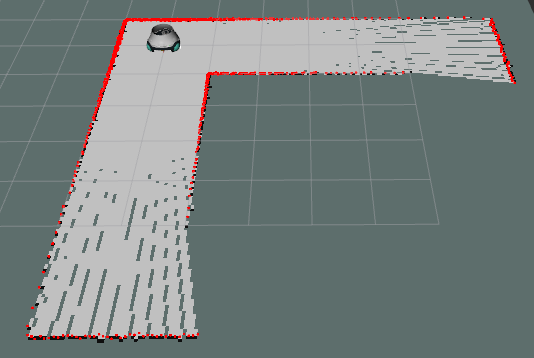
\includegraphics[width=.6\linewidth]{rviz_mapping}
    \caption{Running the automated parser node with Gmapping.}
    \label{fig:rviz_mapping}
\end{figure}

\section{Parsing the data}

The data parser is a Python node that will calculate the required metrics. It runs alongside the SLAM algorithm and constantly import its information. When shut down, the node outputs the desired graphs and metrics. It can be called using the command:

\begin{verbatim}
rosrun cob_bringup_sim pipeline.py
\end{verbatim}

The node keeps executing the following tasks in parallel:

\begin{itemize}
    \item Republishes the ground truth from the ground truth topic (\texttt{/base\_pose\_ground\_truth}, as described in \prettyref{sec:collecting_data}) and republishes it as a tf, since it's easier to do transformations on.
    \item Reads the tf topic and stores a new pose into a pose history whenever the SLAM pose is updated, as well as the ground truth pose.
    \item Collects data from CPU Usage and Memory Usage with the interval of 0.1 seconds.
\end{itemize}

When the node is shutdown, the following tasks are executed:

\begin{itemize}
    \item The pose history is plotted alongside the ground truth.
    \item The squared pose error is calculated according to \prettyref{eq:error_squared}.
    \item The displacement pose error is calculated according to \prettyref{eq:displacement}.
    \item The CPU and Memory usage are plotted over time, using \texttt{psutil} library \cite{psutil}.
    \item The summary is generated including: the average CPU usage, average Memory usage, translation displacement error, rotation displacement error, translation squared error, rotational squared error.
\end{itemize}

\section{Exporting the map}

The map can be exported using the the \texttt{map\_saver} node from the package \texttt{map\_server}. To export the map, simply call the node with the option \texttt{-f} and the map name.

\begin{verbatim}
rosrun map_server map_saver -f map_name
\end{verbatim}

Since Cartographer uses a different approach for generating submaps, the data has to be saved as a \texttt{.pbstream} first to generate the full map. To generate the map, we first have to tell the node to finish the trajectory calling the \texttt{/finish\_trajectory} service. Then, we export the \texttt{.pbstream} file and use it to generate the map. The following sequence of commands represent this process:

\begin{verbatim}
rosservice call /finish_trajectory 0
rosservice call /write_state "filename: '${HOME}/file.pbstream'"
rosrun cartographer_ros cartographer_pbstream_to_ros_map 
       -pbstream_filename ${HOME}/file.pbstream
\end{verbatim}

Because the resulting map doesn't always have the right size (approximately same as the ground truth map), we have to crop the empty gray areas before running the map comparisons. We also want to convert from \texttt{.pgm} saved automatically to \texttt{.png} that the algorithm expects. To do that, we simply call the conversion function from ImageMagick. Why the image is rotated 90 degrees is explained in the next section.

\begin{verbatim}
convert -rotate 90 map_name.pgm -trim map_name.png
\end{verbatim}

\section{Running ICP on resulting map}

Once the map is saved, we have both the reference map and the generated map, as shown in \prettyref{fig:reference_map_icp}. We can then run an algorithm to align the maps properly, as suggested by \citeauthor{santos2013evaluation}.

\begin{figure}[!ht]
     \centering
     \subfloat[][]{
\includegraphics[width=.3\linewidth]{test1_cropped}\label{subfig:test1_cropped}}
     \hspace{2cm}
     \subfloat[][]{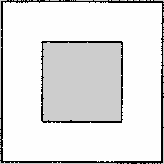
\includegraphics[width=.3\linewidth]{gmapping_test1}\label{subfig:test1_gmapping}}
     \caption{Ground truth (left) and SLAM generated map (right).}
     \label{fig:reference_map_icp}
\end{figure}

First, both maps are imported as a point cloud, each pixel representing a point in space, as shown in \prettyref{fig:point_cloud}. As you can probably tell, the image is twisted 90 degrees counter-clockwise when being read by the algorithm. This happens because the coordinate system for images is not the same as the Cartesian coordinate system.

\begin{figure}[!ht]
     \centering
     \subfloat[][]{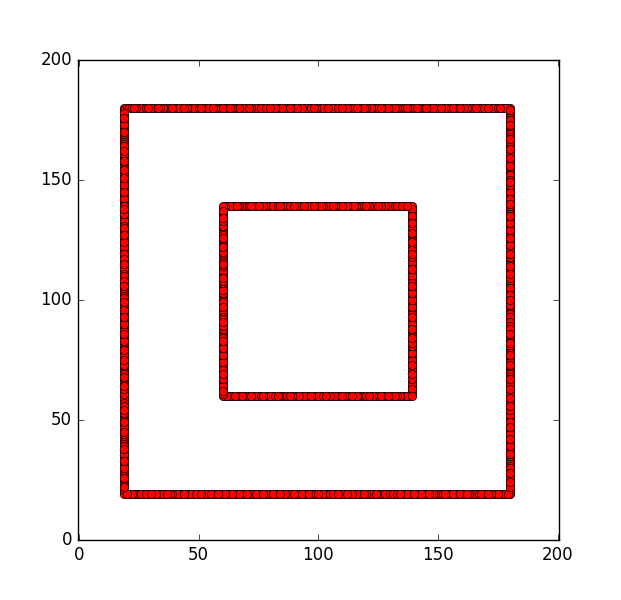
\includegraphics[width=.45\linewidth]{original_pcl}\label{subfig:original_pcl}}
     \hspace{0cm}
     \subfloat[][]{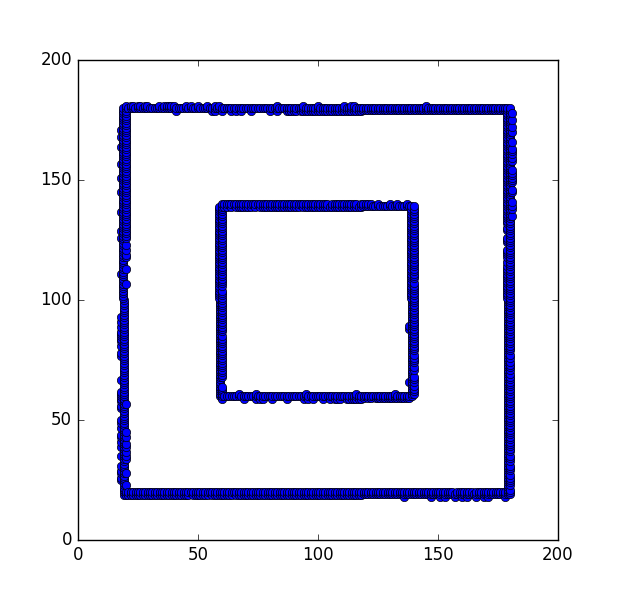
\includegraphics[width=.45\linewidth]{map_pcl}\label{subfig:map_pcl}}
     \caption{Ground truth (left) and SLAM generated map (right) represented in point clouds.}
     \label{fig:point_cloud}
\end{figure}

ICP, or Iteractive Closest Point, is a state-of-the-art way of aligning 3D meshes. It works by finding the transformation that best aligns two distinct point clouds minimizing the error distance between them. For more information about ICP, refer to \citeauthor{besl1992method}.

The ICP algorithm used is the one provided by \citeauthor{flannigan2019}. It will calculate the transformation that best aligns the two maps shown in \prettyref{fig:point_cloud}. With the maps aligned, we then use the following equation to calculate the error metric, where P is the number of points in \figurename~\ref{subfig:map_pcl}, $p_i$ represents one point in the data set and $p_i^*$ is the nearest neighbour of $p_i$ in the dataset shown on \figurename~\ref{subfig:original_pcl}.

\begin{equation}
\epsilon(\text{map}) = \frac{1}{P} \sum_{i=1}^P dist(p_i - p_i^*(p_i))^2
\end{equation}

The aligned point cloud can be seen on \prettyref{fig:alignment_pcl}. To do that, we simply call the node launcher with the desired map and algorithm.

\begin{verbatim}
roslaunch cob_bringup_sim icp_map_comparison.launch map:=test1 slam:=gmapping
\end{verbatim}

\begin{figure}[!ht]
    \centering
    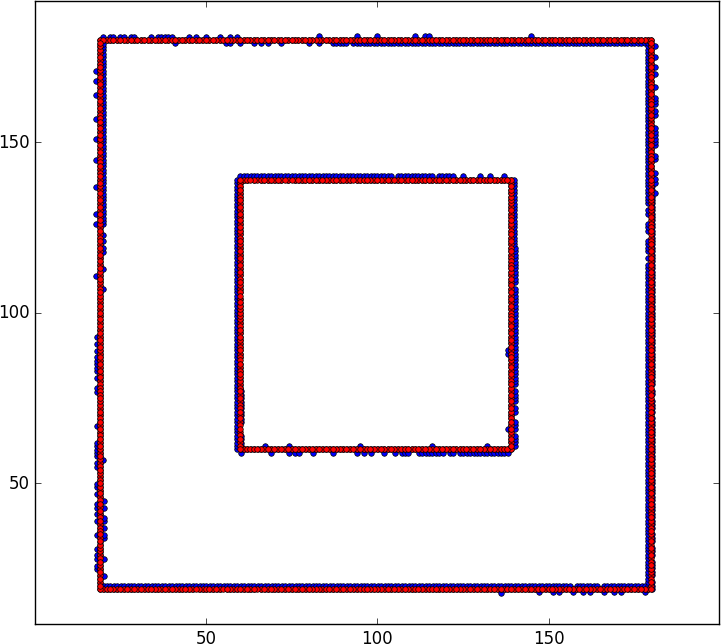
\includegraphics[width=0.45\linewidth]{alignment_pcl}
    \caption{Alignment of point clouds from \prettyref{fig:point_cloud}.}
    \label{fig:alignment_pcl}
\end{figure}

\section{Comparing free space} \label{sec:free_space}

As important as placing the walls in the correct spots, metric that will be checked using ICP, is modeling free space correctly, where the robot can move. This is done by each algorithm by setting the pixels that are free as white. Those white pixels can be counted and checked against the free space in the original map. Since we only want a measurement of scale, we can use the following formula, where $w_o$ is the amount of white pixels in the original image and $w_m$ is the amount of pixels in the map generated by SLAM:

\begin{equation}
\epsilon(\text{space}) = \frac{w_o - w_m}{w_o} \times 100
\end{equation}

The signal of the result will also give indications about the mapping. If it is positive, it means that the original map has more white pixels than the mapped result, meaning the SLAM was more conservative and mapped less space than there is available. If it's negative, the algorithm actually mapped spaced that is not there, meaning the navigation layer will later on have to deal with this problem.
\chapter{Results}\label{chp:results}
\chapter{Conclusions}\label{chp:conclusoes}



%%%%%%%%%%%%%%%%%%%%%%%%%%
%%Elementos Pós-Textuais%%
%%%%%%%%%%%%%%%%%%%%%%%%%%
%%--------Bibliografia--------
\Bibliografia{bibliografia} % arquivo bibtex com as referências (referenciasbibliograficas.bib)

%%--------Apêndice--------
%% Descomente caso exista a necessidade da inclusão de apêndices
%\apendice % Comando que inclui os apêndices
%\include{7_Apendice/apendice_1}   % Arquivo apendice_1.tex
%\include{7_Apendice/apendice_2}   % Arquivo apendice_2.tex
%%---------------------------------------------------------------

%%--------Anexos-------------------------------------------------
%% Descomente caso exista a necessidade da inclusão de anexos
%\anexo % Comando que inclui os anexos (outros autores)
%\include{8_Anexos/anexo_1}  % Arquivo anexo_1.tex
%\include{8_Anexos/anexo_2}  % Arquivo anexo_2.tex
%%---------------------------------------------------------------

\end{document}
